\chapter{Topics in Differential Calculus}
%Begin Section 3.1
\section{Tangent Lines}
Everyone knows that the Earth is not flat, but \emph{locally}, e.g. in your
immediate vicinity, isn't the Earth \emph{effectively} flat? In other words,
``flat'' is a fairly good approximation of the Earth's surface ``near'' you,
and it simplifies matters enough for you to do some useful things.

This idea of approximating curved shapes by straight shapes is a frequent theme
in calculus. Recall from Chapter 1 that by the Microstraightness Property a
differentiable curve $y = f(x)$ actually \emph{is} a straight line over an
infinitesimal interval, having slope $\dydx$. The extension of that line to all
values of $x$ is called the
\emph{tangent line}\index{tangent line}\index{line!tangent}:\index{line}

\statedefn{defn:tangentline}{
{For a curve $y = f(x)$ that is differentiable at $x =a$, the
\textbf{tangent line} to the curve at the point $P = (a, f(a))$ is the unique
line through $P$ with slope $m = f'(a)$. $P$ is called the
\textbf{point of tangency}\index{point of tangency}. The equation of the tangent
line is thus given by:
\begin{equation}\label{eqn:tangentline}
 y ~-~ f(a) ~=~ f'(a) \cdot (x - a)
\end{equation}
}}

\piccaption[]{\label{fig:tangentline}\quad Tangent line}\parpic[r]{
\begin{tikzpicture}[>=latex,every node/.style={font=\small}]
 \draw[<->,black!60,line width=1pt] (-0.5,2.3) node[above] {$y$} |- (4.5,-0.5)
   node[right] {$x$};
 \draw[linecolor,line width=1.5pt] (0,0) .. controls (2,3) and (3.5,-1) .. (4,2)
  node[inner sep=0pt,outer sep=0pt,shape=coordinate,pos=0.05](A) {}
  node[inner sep=0pt,outer sep=0pt,shape=coordinate,pos=0.22](B) {}
  node[inner sep=0pt,outer sep=0pt,shape=coordinate,pos=0.70](C) {}
  node[inner sep=0pt,outer sep=0pt,shape=coordinate,pos=0.80](s) {}
  node[inner sep=0pt,outer sep=0pt,shape=coordinate,pos=0.92](D) {};
 \node[below] at (B) {$P$};
 \node[below] at (4,0.8) {$y=f(x)$};
 \draw[red,line width=0.6pt] (B) -- +(20:1.7) -- +(200:1.4);
 \fill (B) circle (2.5pt);
 \node[left,align=left] at (1.26,1.25) {tangent\\line};
 \draw[black!60] (1.26,-0.59) -- (1.26,-0.41);
 \node[below] at (1.26,-0.59) {$a$};
 \node[above] at (2.26,1.8) {slope = $f'(a)$};
\end{tikzpicture}}
\picskip{10}
Figure \ref{fig:tangentline} on the right shows the tangent line to a curve
$y = f(x)$ at a point $P$. If you were to look at the curve near $P$ with a
microscope, it would look almost identical to its tangent line through $P$. Why
is this line---of all possible lines through $P$---such a good approximation of
the curve near $P$? It is because at the point $P$ the tangent line and the
curve both have the \emph{same rate of change}, namely, $f'(a)$. So the curve's
values and the line's values change by roughly the same amount slightly away
from $P$ (where the line and curve have the same value), making their values
nearly equal.
\newpage
\begin{exmp}\label{exmp:tangentline1}
 \piccaption[]{\label{fig:tangentline1}}\parpic[r]{\begin{tikzpicture}[every node/.style={font=\small}]
  \draw [black!60,line width=1pt,-latex] (-1.5,0) -- (2.6,0) node [right] {$x$};
  \draw [black!60,line width=1pt,-latex] (0,-1.3) -- (0,3) node [above] {$y$};
  \draw [black!60] (1,0.09) -- (1,-0.09) node[black,below] {$1$};
  \draw [black!60] (0.09,1) -- (-0.09,1) node[black,left] {$1$};
  \draw [black!60] (0.09,-1) -- (-0.09,-1) node[black,left] {$-1$};
  \node [below left] at (0,0) {$0$};
  \draw [linecolor,line width=1.5pt] (-1,1) parabola bend (0,0) (1.7,2.89);
  \draw [red,line width=0.6pt] (0,-1) -- (1.6,2.2);
  \fill (1,1) circle (2.5pt);
  \node [above left] at (1,1) {$(1,1)$};
  \node [right] at (1.7,2.89) {$y = x^2$};
  \node [below right] at (1.2,1.4) {$y = 2x - 1$};
 \end{tikzpicture}
}
\noindent Find the tangent line to the curve $y = x^2$ at $x = 1$.\vspace{1mm}
\par\noindent\emph{Solution:} By formula (\ref{eqn:tangentline}), the equation
of the tangent line is
\begin{displaymath}
 y ~-~ f(a) ~=~ f'(a) \cdot (x - a)
\end{displaymath}
with $a = 1$ and $f(x) = x^2$. So $f(a) = f(1) = 1^2 = 1$. Both the curve
$y = x^2$ and the tangent line pass through the point $(1, f(1)) = (1,1)$. The
derivative of $f(x) = x^2$ is $f'(x) = 2x$, so $f'(a) = f'(1) = 2(1) = 2$, which
is the slope of the tangent line at $(1,1)$. Hence, the equation of the tangent
line is $y - 1 = 2(x - 1)$, or (in
slope-intercept form) $y = 2x - 1$.\vspace{2mm}
\par\noindent The curve and tangent line are shown in
Figure \ref{fig:tangentline1}. Near the point $(1,1)$ the curve and tangent line
are close together, but the separation grows farther from that point, especially
in the negative $x$ direction.
\end{exmp}
\divider
\vspace{3mm}

\parpic[r]{\begin{tikzpicture}[every node/.style={font=\small}]
 \draw[linecolor,line width=1.5pt] (0,0) circle (0.707);
 \draw[red,line width=0.6pt] (0,1) -- (1,0);
 \fill (0.5,0.5) circle (2.2pt);
\end{tikzpicture}
}
In trigonometry you probably learned about tangent lines to circles, where a
tangent line is defined as the unique line that touches the circle at only one
point, as in the figure on the right. In this case the tangent line is always on
one side of the circle, namely, the exterior of the circle; it does not cut
through the interior of the circle. In fact, that definition is a special case
of the calculus definition. In general, though, the tangent line to any other
type of curve will not necessarily be on only one side of the curve, as it was
in Example \ref{exmp:tangentline1}.

\begin{exmp}\label{exmp:tangentline2}
 \piccaption[]{\label{fig:tangentline2}}\parpic[r]{\begin{tikzpicture}[every node/.style={font=\small}]
  \draw [black!60,line width=1pt,-latex] (-2,0) -- (2,0) node [right] {$x$};
  \draw [black!60,line width=1pt,-latex] (0,-1.3) -- (0,1.3) node [above] {$y$};
  \draw [linecolor,line width=1.5pt] (0,0) parabola (1.7,1.1);
  \draw [linecolor,line width=1.5pt] (-1.7,-1.1) parabola[bend at end] (0,0);
  \draw [red,line width=0.6pt] (-1.5,0) -- (1.5,0);
  \fill (0,0) circle (2.5pt);
  \node [below right] at (0,0) {$(0,0)$};
  \node [above left] at (1.7,1.1) {$y = x^3$};
  \node [above] at (-1,0) {$y = 0$};
 \end{tikzpicture}
}
\noindent Find the tangent line to the curve $y = x^3$ at $x = 0$.\vspace{1mm}
\par\noindent\emph{Solution:} Use formula (\ref{eqn:tangentline}) with $a = 0$
and $f(x) = x^3$. Then $f(a) = f(0) = 0^3 = 0$. The derivative of $f(x) = x^3$
is $f'(x) = 3x^2$, so $f'(a) = f'(0) = 3(0)^2 = 0$. Hence, the equation of the
tangent line is ${y - 0 = 0(x - 0)}$, which is
$y = 0$. In other words, the tangent line is
the $x$-axis itself.\vspace{1mm}
\par\noindent As shown in Figure \ref{fig:tangentline2}, the tangent line cuts
through the curve. In general it is possible for a tangent line to intersect the
curve at more than one point, depending on the function.
\end{exmp}
\begin{exmp}\label{exmp:tangentline3}
 \piccaption[]{\label{fig:tangentline3}}\parpic[r]{\begin{tikzpicture}[every node/.style={font=\small}]
  \begin{scope}[color=linecolor,line width=1.5pt,x=4cm/360]
   \draw[black!60,line width=1pt,-latex] (-210,0) -- (210,0) node[right] {$x$};
   \draw[black!60,line width=1pt,-latex] (0,-1.2) -- (0,1.2) node[above] {$y$};
   \pgfplothandlerlineto
   \pgfplotfunction{\x}{-180,-175,...,180}{\pgfpointxy{\x}{sin(\x)}}
   \pgfusepath{stroke}
   \draw[red,line width=0.6pt] (45,1) -- (-45,-1);
   \fill[black] (0,0) circle (2.5pt);
   \node[black,above right] at (90,1) {$y = \sin\,x$};
   \node[black,above] at (45,1) {$y = x$};
   \node[black,below right] at (0,0) {$(0,0)$};
  \end{scope}
 \end{tikzpicture}
}
\noindent Find the tangent line to the curve $y = \sin\,x$ at $x = 0$.\vspace{1mm}
\par\noindent\emph{Solution:} Use formula (\ref{eqn:tangentline}) with $a = 0$
and $f(x) = \sin\,x$. Then $f(a) = f(0) = \sin\,0 = 0$. The derivative of
$f(x) = \sin\,x$ is $f'(x) = \cos\,x$, so $f'(a) = f'(0) = \cos\,0 = 1$. Hence,
the equation of the tangent line is ${y - 0 = 1(x - 0)}$, which is
$y = x$, as in Figure \ref{fig:tangentline3}.
Near $x = 0$, the tangent line $y = x$ is close to the line $y = \sin\,x$, which
was shown in Section 1.3 (namely, $\sin\,\dx = \dx$, so that $\sin\,x \approx x$
for $x \ll 1$).
\end{exmp}
\divider
\newpage
There are several important things to note about tangent lines:
\begin{itemize}
 \item \emph{The slope of a curve's tangent line is the slope of the curve}.\\
  Since the slope of a tangent line equals the derivative of the curve at the
  point of tangency, the \textbf{slope of a curve} at a particular point can be
  defined as the slope of its tangent line at that point.\index{slope of a curve}
  So curves can have varying slopes, depending on the point, unlike straight
  lines, which have a constant slope. An easy way to remember all this is to
  think ``slope = derivative.''
 \item \emph{The tangent line to a straight line is the straight line itself}.\\
  This follows easily from the definition of a tangent line, but is also easy
  to see with the ``slope = derivative'' idea: a straight line's slope (i.e.
  derivative) never changes, so its tangent line---having the same slope---will
  be parallel and hence must coincide with the straight line (since they have
  the points of tangency in common). For example, the tangent line to the
  straight line $y = -3x + 2$ is $y = -3x + 2$ at every point on the straight
  line.
 \item \emph{The tangent line can be thought of as a limit of secant lines}.\\
 A \textbf{secant line}\index{secant line} to a curve is a line that passes
through two points on the curve. Figure \ref{fig:secantline} shows a secant line
$L_{PQ}$ passing through the points $P = (x_0,f(x_0)) $ and $Q = (w,f(w))$ on the
curve $y = f(x)$,

\begin{figure}[h]
 \begin{center}
  \begin{tikzpicture}[>=latex,every node/.style={font=\small}]
  \draw[<->,black!60,line width=1pt] (0,4) node[above] {$y$} |- (6,0) node[right] {$x$};
  \draw[name path=curve,linecolor,line width=1.5pt,shift={(1,4)}] (-90:3) arc (-90:-10:3.5);
  \node[left] at (4.2,3.9) {$y = f(x)$};
  \draw[name path=secant,line width=0.6pt] (4.7, 3.7) -- (1.3,0.5) node[pos=0.0,right] {$L_{PQ}$};
  \fill[black,name intersections={of=curve and secant,by={Q,P}}]
   (P) circle (2.5pt) node[above] {$P$}
   (Q) circle (2.5pt) node[below right] {$Q$};
  \draw[red,line width=0.6pt] (P) -- +(17:2.8) -- +(197:1) node[black,pos=0.0,right] {$T_P$};
  \fill[black] (P) circle (2.5pt);
  \coordinate (x) at ($(0,0)!(P)!(6,0)$);
  \coordinate (y) at ($(0,0)!(P)!(0,4)$);
  \coordinate (w) at ($(0,0)!(Q)!(6,0)$);
  \coordinate (v) at ($(0,0)!(Q)!(0,4)$);
  \draw[black!60] (x) -- +(0,0.09) -- +(0,-0.09) node[black,below] {$x_0$};
  \draw[black!60] (y) -- +(0.09,0) -- +(-0.09,0) node[black,left] {$f(x_0)$};
  \draw[black!60] (w) -- +(0,0.09) -- +(0,-0.09) node[black,below] {$w$};
  \draw[black!60] (v) -- +(0.09,0) -- +(-0.09,0) node[black,left] {$f(w)$};
 \end{tikzpicture} \vspace{-5mm}
 \end{center}
 \caption[]{\quad Secant line $L_{PQ}$ approaching the tangent line $T_P$ as $Q \to P$}
 \label{fig:secantline}
\end{figure}

\par\noindent As the point $Q$ moves along the curve toward $P$, the line $L_{PQ}$
approaches the tangent line $T_P$ at the point $P$, provided the curve is smooth
at $P$ (i.e. $f'(x_0)$ exists). This is because the slope of $L_{PQ}$ is
$(f(w) - f(x_0))/(w - x_0)$, and so
\begin{displaymath}
 \lim_{Q \to P} ~ \left(\text{slope of } L_{PQ}\right) ~=~
 \lim_{w \to x_0} ~\frac{f(w) ~-~ f(x_0)}{w ~-~ x_0} ~=~ f'(x_0) ~=~
 \text{slope of } T_P
\end{displaymath}
which means that as $Q$ approaches $P$ the ``limit'' of the secant line $L_{PQ}$
has the same slope and goes through the same point $P$ as the tangent line $T_P$.
\newpage
 \item \emph{Smooth curves have tangent lines, nonsmooth curves do not.}\\
  For example, think of the absolute value function $f(x) = \abs{x}$. Its graph has a sharp
  edge at the point $(0,0)$, making it nonsmooth there, as shown in Figure
  \ref{fig:tangentnonsmooth}(a) below. There is no real way to define a tangent line at
  $(0,0)$, because as mentioned in Section 1.2, the derivative of $f(x)$ does not exist
  at $x = 0$. The same holds true for curves with cusps, as in Figure
  \ref{fig:tangentnonsmooth}(b).

\begin{figure}[ht]
 \centering
 \subfloat[][ $f(x) = \abs{x}$]{
 \begin{tikzpicture}[scale=0.8,>=latex, every node/.style={font=\small}]
  \draw[->,black!60,line width=1pt] (-3,0) -- (3,0) node[right] {$x$};
  \draw[->,black!60,line width=1pt] (0,0) -- (0,2) node[above] {$y$};
  \draw[linecolor,line width=1.5pt] (-1.8,1.8) -- (0,0) -- (1.8,1.8);
  \draw[red,dashed,line width=0.6pt] (1.6,0.8) -- (-0.6,-0.3);
  \draw[red,dashed,line width=0.6pt] (-1.6,0.4) -- (0.8,-0.2);
  \draw[red,dashed,line width=0.6pt] (-1.6,0) -- (1.6,0);
  \node[below] at (0,0) {$0$}; 
  \node[above] at (1.8,1.8) {$y = \abs{x}$};
 \end{tikzpicture}}
 \qquad\qquad
 \subfloat[][ Curve with a cusp]{
  \begin{tikzpicture}[scale=0.8,>=latex, every node/.style={font=\small}]
   \draw[linecolor,line width=1.5pt] (-2,-1) parabola bend (-1,1) (0,0)
     parabola bend (2,2) (4,1);
   \draw[red,dashed,line width=0.6pt] (2,1) -- (-1,-0.5);
   \draw[red,dashed,line width=0.6pt] (-0.6,0.2) -- (0.9,-0.3);
  \node[right] at (4,1) {$y = f(x)$};
 \end{tikzpicture}}
 \caption[]{\quad Nonsmooth curves: no tangent line at the nonsmooth points}
 \label{fig:tangentnonsmooth}
\end{figure}

\par\noindent Many lines go through the point of nonsmoothness, some of
which are indicated by the dashed lines in the above figures, but none of
them can be the tangent line. Sharp edges and cusps have to be ``smoothed out''
to have a tangent line.
\end{itemize}
\divider
\vspace{3mm}

As a point moves along a smooth curve, the corresponding tangent lines to the
curve make varying angles with the positive $x$-axis---the angle is thus a
function of $x$. Let $\phi = \phi(x)$ be the smallest angle that the tangent
line $L$ to a curve $y = f(x)$ makes with the positive $x$-axis, so that
$-90\Degrees < \phi(x) <90\Degrees$ for all $x$ (see Figure \ref{fig:tangentangle}).

\begin{figure}[ht]
 \centering
 \begin{tikzpicture}[>=latex, every node/.style={font=\small}]
  \draw [->,shift={(2.246,0.55)}] (0:1.3) arc (0:36.1:1.3);
  \draw [black!60,line width=1pt,-latex] (-7.0,0.55) -- (6,0.55) node [right] {$x$};
  \draw [black!60] (-5,0.55) -- (-5,0.45) node [below] {$x_1$};
  \draw [black!60] (0,0.55) -- (0,0.45) node [below] {$x_2$};
  \draw [black!60] (3,0.55) -- (3,0.45) node [below] {$x_3$};
  \draw [black!60,line width=1pt,-latex] (-6.5,-0.74) -- (-6.5,1.3) node [above] {$y$};
  \draw [linecolor,line width=1.5pt] (-5.5,1.5) parabola[bend at end] (0,0);
  \draw [linecolor,line width=1.5pt] (0,0) parabola (3.5,1.5);
  \draw [->,shift={(-3.61,0.55)}] (-0.5:2.23) arc (-0.5:-26.37:2.23);
  \node [left] at (3.0,1.5) {$y = f(x)$};
  \draw [red,line width=0.6pt] (-1.05,0) -- (1.45,0);
  \fill (0,0) circle (2.5pt);
  \node [below] at (1.45,0) {$L$};
  \node [below] at (0.3,0) {$\phi(x_2)=0\Degrees$};
  \draw [red,line width=0.6pt] (3.5,1.46) -- (2,0.37);
  \fill (3.0,1.1) circle (2.5pt);
  \node [below right] at (2,0.37) {$L$};
  \node at (3.05,0.75) {$\phi(x_3)$};
  \draw [red,line width=0.6pt] (-5.5,1.487) -- (-1.0,-0.744);
  \fill (-5,1.24) circle (2.5pt);
  \node [below left] at (-1.0,-0.744) {$L$};
  \node at (-1.9,0) {$\phi(x_1)$};
 \end{tikzpicture}
 \caption[]{\quad The angle $\phi(x)$ between the tangent line and positive $x$-axis}
 \label{fig:tangentangle}
\end{figure}

\parpic[r]{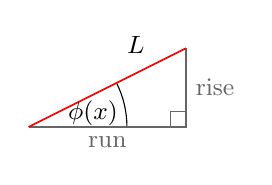
\begin{tikzpicture}[every node/.style={font=\small}]
 \draw (0:1.25) arc (0:26.5:1.25);
 \draw[black!60] (0,0) -- (2,0) node[midway,below] {run} -- (2,1) node[midway,right] {rise};
 \draw[red,line width=0.6pt] (0,0) -- (2,1) node[black,pos=0.8,above left] {$L$};
 \node[right] at (0.38,0.17) {$\phi(x)$};
 \draw[black!60] (1.8,0) -- (1.8,0.2) -- (2,0.2);
\end{tikzpicture}}
As Figure \ref{fig:tangentangle} shows, $-90\Degrees < \phi(x) < 0\Degrees$ when
the tangent line $L$ has negative slope, $0\Degrees < \phi(x) < 90\Degrees$ when
$L$ has positive slope, and $\phi(x)=0\Degrees$ when $L$ is horizontal (i.e. has
zero slope). The slope of a line is usually defined as the rise divided by the
run in a right triangle, as shown in the figure on the right. The figure shows
as well that by definition of the tangent of an angle, $\tan\,\phi(x)$ also
equals the rise (opposite) over run (adjacent). Thus, since the slope of $L$ is
$f'(x)$, this means that $\tan\,\phi(x) = f'(x)$. In other words:
\index{angle of tangent line}\index{tangent line!angle of}

\statethm{thm:tangentangle}{
{The tangent line to a curve $y=f(x)$ makes an angle $\phi(x)$ with the positive
 $x$-axis, given by
\begin{equation}\label{eqn:tangentangle}
\phi(x) ~=~ \tan^{-1} f'(x) ~.
\end{equation}}
}

\begin{exmp}\label{exmp:tangentangle}
\parpic[r]{\begin{tikzpicture}[>=latex,every node/.style={font=\small},domain=-1.9:0.3]
 \draw [->,black!60,line width=1pt] (0,0) -- (0,2) node[pos=1.0,above] {$y$};
 \draw [->,shift={(-1,0)}] (0:1.05) arc (0:36.1:1.05);
 \draw [->,black!60,line width=1pt] (-2,0) -- (1.2,0) node[pos=1.0,right] {$x$};
 \draw[linecolor,line width=1.5pt] plot (\x,{exp(2.0*\x)});
 \node[above right] at (0.3,1.8) {$y = e^{2x}$};
 \fill (-0.5,0.3679) circle (2.5pt);
 \node[above left] at (-0.5,0.3679) {$\left(-\frac{1}{2},\frac{1}{e}\right)$};
 \draw[red,line width=0.6pt] (-1,0) -- (0.5,1.104);
 \node[right] at (0.5,1.104) {$L$};
 \node at (-0.23,0.2) {$\phi$};
\end{tikzpicture}
}
\noindent Find the angle $\phi$ that the tangent line to the curve $y=e^{2x}$ at
$x = -\frac{1}{2}$ makes with the positive $x$-axis, such that $-90\Degrees <
\phi < 90\Degrees$.\vspace{1mm}
\par\noindent\emph{Solution:} The angle is $\phi =
\phi(-1/2) = \tan^{-1} f`(-1/2)$, where
$f(x) = e^{2x}$. Since $f'(x) = 2e^{2x}$, then
\[
\phi ~=~ \phi(-1/2) ~=~ \tan^{-1} f`(-1/2)
 ~=~ \tan^{-1} 2e^{-1} ~=~ \tan^{-1} 0.7358 ~=~ 36.3\Degrees ~.
\]
The figure on the right shows the tangent line $L$ to the curve at
$x = -\frac{1}{2}$ and the angle $\phi$.
\end{exmp}\vspace{-1mm}
\divider
\vspace{2mm}

\piccaption[]{\label{fig:normalline}\quad Normal line $N$}\parpic[r]{
\begin{tikzpicture}[>=latex,every node/.style={font=\small}]
 \draw[<->,black!60,line width=1pt] (-0.5,2.3) node[above] {$y$} |- (4,0)
   node[right] {$x$};
 \draw[linecolor,line width=1.5pt] (0.1,0.1) .. controls (2,3) and (3.5,0) .. (3.7,2)
  node[inner sep=0pt,outer sep=0pt,shape=coordinate,pos=0.05](A) {}
  node[inner sep=0pt,outer sep=0pt,shape=coordinate,pos=0.22](B) {}
  node[inner sep=0pt,outer sep=0pt,shape=coordinate,pos=0.70](C) {}
  node[inner sep=0pt,outer sep=0pt,shape=coordinate,pos=0.80](s) {}
  node[inner sep=0pt,outer sep=0pt,shape=coordinate,pos=0.92](D) {};
 \node[below] at (1.22,1) {$P$};
 \node[below] at (3.45,1.28) {$y=f(x)$};
 \draw[black!60,shift={(B)},rotate=22] (0.2,0) -- (0.2,0.2) -- (0,0.2);
 \draw[red,line width=0.6pt] (B) -- +(22:1.7) -- +(202:1.3) node[right,black,pos=0] {$L$};
 \draw[green!80,line width=0.6pt] (B) -- +(112:1.13) -- +(292:1.1) node[above,black,pos=0] {$N$};
 \fill (B) circle (2.5pt);
 \node[above,align=left] at (0.25,1.35) {normal\\line};
 \draw[black!60] (1.26,-0.09) -- (1.26,0.09);
 \node[below] at (1.26,-0.09) {$a$};
 \node[above,align=left] at (2.76,1.8) {tangent\\line};
\end{tikzpicture}}
\noindent You learned about perpendicular lines in elementary geometry. Figure
\ref{fig:normalline} shows the natural way to define how a line $N$ can be
perpendicular to a \emph{curve} $y=f(x)$ at a point $P$ on the curve: the line
is perpendicular to the tangent line of the curve at $P$. Call this line $N$ the
\textbf{normal line}\index{normal line}\index{line!normal} to the curve at $P$.
Since $N$ and $L$ are perpendicular, their slopes are negative reciprocals of
each other (provided neither slope is 0). The equation of the normal line
follows easily:
 
\statethm{thm:normalline}{
{The equation of the normal line to a curve $y=f(x)$ at a point $P=(a,f(a))$ is

\begin{equation}\label{eqn:normalline}
y ~-~ f(a) ~=~ -\frac{1}{f'(a)} \cdot (x ~-~ a) \quad\text{if $f'(a) \ne 0$.}
\end{equation}
If $f'(a) = 0$, then the normal line is vertical and is given by $x = a$.}
}

\begin{exmp}\label{exmp:normalline}
Find the normal line to the curve $y = x^2$ at $x = 1$.
(Note: This is the curve from Example \ref{exmp:tangentline1}.)\vspace{1mm}
\par\noindent\emph{Solution:} The equation of the normal line is
\begin{displaymath}
 y ~-~ f(a) ~=~ -\frac{1}{f'(a)} \cdot (x - a)
\end{displaymath}
with $a = 1$, $f(x) = x^2$, and $f'(x) = 2x$. So $f(a) = 1$ and $f'(a) = 2$.
Hence, the equation of the normal line is
$y - 1 = -\frac{1}{2}(x - 1)$, or (in
slope-intercept form)
$y = -\frac{1}{2}x + \frac{3}{2}$.
\end{exmp}
\divider
\newpage
\vspace{3mm}
\startexercises\label{sec3dot1}
{\small
\probs{A}
\par\noindent For Exercises 1-12, find the equation of the tangent line to the
curve $y = f(x)$ at $x = a$.
\begin{enumerate}[\bfseries 1.]
 \begin{multicols}{3}
  \item $f(x) ~=~ x^2 ~+~ 1$; at $x = 2$
  \item $f(x) ~=~ x^2 ~-~ 1$; at $x = 2$
  \item $f(x) ~=~ -x^2 ~+~ 1$; at $x = 3$
 \end{multicols}
 \begin{multicols}{3}
  \item $f(x) ~=~ 1$; at $x = -1$
  \item $f(x) ~=~ 4x$; at $x = 1$
  \item $f(x) ~=~ e^x$; at $x = 0$
 \end{multicols}
 \begin{multicols}{3}
  \item $f(x) ~=~ x^2 ~-~ 3x ~+~ 7$; at $x = 2\vphantom{\dfrac{x ~+~ 1}{x ~-~ 1}}$
  \item $f(x) ~=~ \dfrac{x ~+~ 1}{x ~-~ 1}$; at $x = 0$
  \item $f(x) ~=~ (x^3 ~+~ 2x ~-~ 1)^3$; at $x = -1\vphantom{\dfrac{x ~+~ 1}{x ~-~ 1}}$
 \end{multicols}
 \begin{multicols}{3}
  \item $f(x) ~=~ \tan\,x$; at $x = 0$
  \item $f(x) ~=~ \sin\,2x$; at $x = 0$
  \item $f(x) ~=~ \sqrt{1 ~-~ x^2}$; at $x = 1/\sqrt{2}$
 \end{multicols}
 \item Find the equations of the tangent lines to the curve
  $y = x^3 - 2x^2 + 4x + 1$  which are parallel to the line $y = 3x - 5$.
 \item Draw an example of a curve having a tangent line that intersects the
 curve at more than one point.
\suspend{enumerate}
\noindent For Exercises 15-17, find the angle $\phi$ that the tangent line to the
curve $y=f(x)$ at $x=a$ makes with the positive $x$-axis, such that
$-90\Degrees < \phi < 90\Degrees$.
\resume{enumerate}[{[\bfseries 1.]}]
 \begin{multicols}{3}
  \item $f(x) ~=~ x^2$; at $x = 2$
  \item $f(x) ~=~ \cos\,2x$; at $x = \pi/6$
  \item $f(x) ~=~ x^2 ~+~ 2x ~-~ 3$; at $x = -1$
 \end{multicols}
 \item Show that if $\phi(x)$ is the angle that the tangent line to a curve
  $y = f(x)$ makes with the positive $x$-axis such that
  $0\Degrees \le \phi(x) < 180\Degrees$, then
\[
\phi(x) ~=~
\begin{cases}
~\cos^{-1} \left(\dfrac{1}{\sqrt{1 ~+~ (f'(x))^2}}\right) & \text{when $f'(x) \ge 0$}\\[12pt]
~\cos^{-1} \left(\dfrac{-1}{\sqrt{1 ~+~ (f'(x))^2}}\right) & \text{when $f'(x) < 0$.}
\end{cases}
\]
\emph{(Hint: Draw a right triangle.)}
\suspend{enumerate}
\noindent For Exercises 19-21, find the angle $\phi$ that the tangent line to the
curve $y=f(x)$ at $x=a$ makes with the positive $x$-axis, such that
$0\Degrees \le \phi < 180\Degrees$.
\resume{enumerate}[{[\bfseries 1.]}]
 \begin{multicols}{3}
  \item $f(x) ~=~ x^2$; at $x = -1$
  \item $f(x) ~=~ e^{-x}$; at $x = 1$
  \item $f(x) ~=~ \ln 2x$; at $x = 10$
 \end{multicols}
\suspend{enumerate}
\par\noindent For Exercises 22-24, find the equation of the normal line to the
curve $y = f(x)$ at $x = a$.
\resume{enumerate}[{[\bfseries 1.]}]
 \begin{multicols}{3}
  \item $f(x) ~=~ \sqrt{x}$; at $x = 4$
  \item $f(x) ~=~ x^2 ~+~ 1$; at $x = 2$
  \item $f(x) ~=~ x^2 ~-~ 7x ~+~ 4$; at $x = 3$
 \end{multicols}
\item Find the equations of the normal lines to the curve
  $y = x^3 - 2x^2 - 11x + 3$ which have a slope of $-\frac{1}{4}$.
\suspend{enumerate}
\probs{B}
\resume{enumerate}[{[\bfseries 1.]}]
 \item Show that the area of the triangle formed by the $x$-axis, the $y$-axis, and the
tangent line to the curve $y = 1/x$ at any point $P$ is constant (i.e. the area is the
same for all $P$).
 \item For a constant $a > 0$, let $P$ be a point on the curve $y = ax^2$, and let $Q$
be the point where the tangent line to the curve at $P$ intersects the $y$-axis. Show that
the $x$-axis bisects the line segment $\overline{PQ}$.
 \item Let $P$ be a point on the curve $y = 1/x$ in the first quadrant, and let $Q$ be the
point where the tangent line to the curve at $P$ intersects the $x$-axis. Show that the
triangle $\Delta\,POQ$ is isosceles, where $O$ is the origin.
\end{enumerate}}
\newpage
%Begin Section 3.2
\section{Limits: Formal Definition}
So far only the intuitive notion of a limit\index{limit} has been used, namely:
\statecomment{A real number $L$ is the limit of $f(x)$ as $x$ approaches $a$ if the values
of $f(x)$ can be made \emph{arbitrarily} close to $L$ by picking values of $x$
\emph{sufficiently} close to $a$.}

\noindent That notion can be put in terms of a formal definition as follows:

\statedefn{defn:limit}{
 Let $L$ and $a$ be real numbers. Then $L$ is the \textbf{limit} of a function $f(x)$ as $x$ approaches
 $a$, written as
 \begin{displaymath}
  \lim_{x \to a} ~f(x) ~=~ L ~,
 \end{displaymath}
 if for any given number $\epsilon > 0$, there exists a number $\delta > 0$, such that
 \begin{displaymath}
  \abs{f(x) - L} < \epsilon \quad\text{whenever}\quad 0 < \abs{x - a} < \delta ~.
 \end{displaymath}
}

\noindent A visual way of thinking of this definition is shown in Figure
\ref{fig:limit} below:

\begin{figure}[ht]
 \begin{center}
  \begin{tikzpicture}[every node/.style={font=\small},scale=1.2]
   \usetikzlibrary{arrows}
   \usetikzlibrary{decorations.pathreplacing}
   \fill [fill=fillcolor] (2.2,0) -- (2.2,1) -- (0,1) -- (0,1.8) -- (3.6,1.8) -- (3.6,0) -- (2.2,0);
   \draw[latex-latex,black!60,line width=1pt] (0,2.6) node[above] {$y$} |- (5,0) node[right] {$x$};
   \draw [linecolor,line width=1.5pt] (0.2,0.5) parabola (4,2.2);
   \node [above] at (4,2.2) {$y = f(x)$};
   \node [below] at (2.2,0) {$a-\delta$};
   \node at (2.24,0) {$($};
   \node [below] at (2.9,0) {$a\vphantom{\delta}$};
   \node [below] at (3.6,0) {$a+\delta$};
   \node at (3.56,0) {$)$};
   \node [left] at (0,2) {$L+\epsilon$};
   \node [left] at (0,1.365) {$L$};
   \node [left] at (0,0.73) {$L-\epsilon$};
   \draw [dashed] (1.6,0) -- (1.6,0.73);
   \draw [dashed] (0,0.73) -- (3.8,0.73);
   \draw [dashed] (2.9,0.07) -- (2.9,1.365);
   \draw [dashed] (0,1.365) -- (2.9,1.365);
   \draw [dashed] (3.8,0) -- (3.8,2);
   \draw [dashed] (0,2) -- (3.8,2);
   \draw [dotted] (2.2,0) -- (2.2,1);
   \draw [dotted] (3.6,0) -- (3.6,1.8);
   \draw [dotted] (0,1) -- (2.2,1);
   \draw [dotted] (0,1.8) -- (3.6,1.8);
   \fill (2.9,1.365) circle (2.5pt);
   \draw (2.9,0) circle (2pt);
   \draw[decorate,decoration={brace,mirror,amplitude=4pt,raise=15pt}] (2.2,0) -- (3.6,0);
   \node [below] at (2.9,-0.7) {$0 < \abs{x-a} < \delta$};
   \draw[decorate,decoration={brace,amplitude=4pt,raise=28pt}] (0,0.73) -- (0,2);
   \node [left] at (-1.3,1.365) {$\abs{f(x)-L} < \epsilon$};
   \draw [white] (7,0) -- (8,0);
  \end{tikzpicture}\vspace{-6mm}
 \end{center}
 \caption[]{\quad $\displaystyle\lim_{x \to a} ~f(x) = L$}
 \label{fig:limit}
\end{figure}\vspace{-2mm}

\par\noindent Figure \ref{fig:limit} says that for any interval around $L$ on
the $y$-axis, you will be able to find at least one small interval around
$x = a$ (but excluding $a$) on the $x$-axis that the function $y=f(x)$ maps
completely inside that interval on the $y$-axis. Choosing smaller intervals
around $L$ on the $y$-axis could force you to find smaller intervals around
$a$ on the $x$-axis.

In Figure \ref{fig:limit}, $f(x)$ is made arbitrarily close to $L$
(within any distance $\epsilon > 0$) by picking $x$ sufficiently close to $a$
(within some distance $\delta > 0$). Since $0 < \abs{x - a} < \delta$ means that
$x = a$ itself is excluded, the solid dot at $(a,L)$ could even be a hollow dot.
That is, $f(a)$ does not have to equal $L$, or even be defined; $f(x)$ just
needs to \emph{approach} $L$ as $x$ approaches $a$. Thus--perhaps
counter-intuitively---the existence of the limit does not actually depend on
what happens \emph{at} $x=a$ itself.
\newpage
\begin{exmp}\label{exmp:limx}
 Show that $\displaystyle\lim_{x \to a} ~x = a\,$ for any real number $a$.\vspace{1mm}
 \par\noindent\emph{Solution:} Though the limit is obvious, the following
``epsilon-delta'' proof shows how to use the formal definition. The idea is to
let $\epsilon > 0$ be given, then ``work backward'' from the inequality
$\abs{f(x)-L} < \epsilon$ to get an inequality of the form $\abs{x-a} < \delta$,
where $\delta > 0$ usually depends on $\epsilon$. In this case the limit is 
$L = a$ and the function is $f(x) = x$, so since
 \begin{align*}
  \abs{f(x)-a} < \epsilon \quad&\Leftrightarrow\quad \abs{x-a} < \epsilon ~,\\
  \intertext{then choosing $\delta = \epsilon$ means that}
  0 < \abs{x-a} < \delta \quad&\Rightarrow\quad \abs{x-a} < \epsilon
  \quad\Rightarrow\quad \abs{f(x)-a} < \epsilon ~,
 \end{align*}
 which by definition means that $\displaystyle\lim_{x \to a} ~x = a$.
\end{exmp}
\divider
\vspace{3mm}

Calculating limits in this way might seem silly since---as in Example
\ref{exmp:limx}---it requires extra effort for a result that is obvious. The
formal definition is used most often in proofs of general results and theorems.
For example, the rules for limits---listed in Section 1.2---can be proved by
using the formal definition.

\begin{exmp}\label{exmp:limsum}
 Suppose that $\displaystyle\lim_{x \to a} f(x)$ and
 $\displaystyle\lim_{x \to a} g(x)$ both exist. Show that
 \[
 \lim_{x \to a} ~(f(x) + g(x)) ~=~
  \left(\lim_{x \to a} ~f(x)\right) ~+~
  \left(\lim_{x \to a} ~g(x)\right)
\]
\par\noindent\emph{Solution:} Let $\displaystyle\lim_{x \to a} f(x) = L_1$ and
$\displaystyle\lim_{x \to a} g(x) = L_2$. The goal is to show that
$\displaystyle\lim_{x \to a} ~(f(x) + g(x)) = L_1 + L_2$. So let $\epsilon > 0$.
Then $\epsilon/2 > 0$, and so by definition there exist numbers
$\delta_1 > 0$ and $\delta_2 > 0$ such that
\begin{align*}
 0 < \abs{x - a} < \delta_1 \quad&\Rightarrow\quad \abs{f(x) ~-~ L_1} < \epsilon/2~\text{, and}\\
 0 < \abs{x - a} < \delta_2 \quad&\Rightarrow\quad \abs{g(x) ~-~ L_2} < \epsilon/2 ~.
\end{align*}
Now let $\delta = \min(\delta_1, \delta_2)$. Then $\delta > 0$ and
\begin{align*}
 0 < \abs{x - a} < \delta \quad&\Rightarrow\quad
 0 < \abs{x - a} < \delta_1 \quad\text{and}\quad 0 < \abs{x - a} < \delta_2\\
 &\Rightarrow\quad \abs{f(x) ~-~ L_1} < \epsilon/2 \quad\text{and}\quad
  \abs{g(x) ~-~ L_2} < \epsilon/2
\end{align*}
Since $\abs{A+B} \le \abs{A} + \abs{B}$ for all real numbers $A$ and $B$, then
\[
 \abs{f(x) ~+~ g(x) ~-~ (L_1 + L_2)} ~=~
  \abs{(f(x) ~-~ L_1) ~+~ (g(x) ~-~ L_2)} ~\le~
  \abs{f(x) ~-~ L_1} ~+~ \abs{g(x) ~-~ L_2}
\]
and thus
\[
 0 < \abs{x-a} < \delta \quad\Rightarrow\quad
 \abs{f(x) ~+~ g(x) ~-~ (L_1 + L_2)} ~<~ \epsilon/2 ~+~ \epsilon/2 ~=~ \epsilon
\]
which by definition means that $\displaystyle\lim_{x \to a} ~(f(x) + g(x)) = L_1 + L_2$.
\quad\checkmark
\end{exmp}
\divider
\newpage
The proofs of the other limit rules are similar.\footnote{For example, see
Section 2.2 in \textsc{Protter, M.H. and C.B. Morrey}, \emph{A First Course in
Real Analysis}, New York: Springer-Verlag, 1977.} In general, using the formal
definition will not be necessary for evaluating limits of specific
functions---in many cases a simple analysis of the function is all that is
needed, often from its graph.

\begin{exmp}\label{exmp:limsimple}
 \piccaption[]{\label{fig:limsimple}}\parpic[r]{\begin{tikzpicture}[every node/.style={font=\small}]
  \draw [black!60,line width=1pt,-latex] (-1.5,0) -- (2.6,0) node [right] {$x$};
  \draw [black!60,line width=1pt,-latex] (0,0) -- (0,3) node [above] {$y$};
  \draw [black!60] (1,0.09) -- (1,-0.09) node[black,below] {$1$};
  \draw [black!60] (0.09,1) -- (-0.09,1) node[black,below left] {$1$};
  \draw [black!60] (0.09,2) -- (-0.09,2) node[black,left] {$2$};
  \node [below] at (0,0) {$0$};
  \draw [linecolor,line width=1.5pt] (-1,1) -- (1,1) -- (2.3,2.3);
  \filldraw [fill=white] (1,1) circle (2.5pt);
  \fill (1,2) circle (2.5pt);
  \node [above] at (2.3,2.3) {$y = f(x)$};
 \end{tikzpicture}
}
\noindent Evaluate $\displaystyle\lim_{x \to 1}~f(x)$ for the following function:
\[
 f(x) ~=~ \begin{cases}
           ~x & \text{if } x > 1\\
           ~2 & \text{if } x = 1\\
           ~1 & \text{if } x < 1
          \end{cases}
\]
\par\noindent\emph{Solution:} From the graph of $f(x)$ in Figure \ref{fig:limsimple},
it is clear that as $x$ approaches $1$ from the right (i.e. for $x > 1$) $f(x)$
approaches $1$ along the line $y = x$, whereas as $x$ approaches $1$ from the
left (i.e. for $x < 1$) $f(x)$ approaches $1$ along the horizontal line $y = 1$.
Thus, $\displaystyle\lim_{x \to 1}~f(x) = 1~$.\\
Note that the limit did not depend on the value of $f(x)$ at $x = 1$.
\end{exmp}
\divider
\vspace{3mm}

As Example \ref{exmp:limsimple} shows, what matters for a limit is what happens
to the value of $f(x)$ as $x$ gets
\emph{near} $a$, not at $x=a$ itself. Figure \ref{fig:lims}(a) below shows how
as $x$ approaches $a$, $f(x)$ approaches a number different from $f(a)$. Figure
\ref{fig:lims}(b) shows that $x=a$ does not even need to be in the domain of
$f(x)$, i.e. $f(a)$ does not have to be defined. So it will not always
be the case that $\displaystyle\lim_{x \to a} ~f(x) = f(a)$.

\begin{figure}[ht]
 \centering
 \subfloat[][ $\;\displaystyle\lim_{x \to a} ~f(x) = L \ne f(a)$]{
 \begin{tikzpicture}[every node/.style={font=\small}]
  \usetikzlibrary{arrows}
  \draw[latex-latex,black!60,line width=1pt] (0,2.6) node[above] {$y$} |- (5,0) node[right] {$x$};
  \draw [linecolor,line width=1.5pt] (0.2,0.5) parabola (4,2.2);
  \node [right] at (4,2.2) {$y = f(x)$};
  \node [below] at (2.9,0) {$a$};
  \node [left] at (0,1.365) {$L$};
  \node [left] at (0,2) {$f(a)$};
  \fill (2.9,1.365) circle (2.5pt);
  \draw [dotted] (0,1.365) -- (2.9,1.365);
  \draw [dotted] (2.9,0) -- (2.9,2);
  \filldraw [fill=white] (2.9,1.365) circle (2.5pt);
  \fill (2.9,2) circle (2.5pt);
  \node [above] at (2.9,2) {$(a,f(a))$};
  \draw [dotted] (0,2) -- (2.9,2);
 \end{tikzpicture}}
 \qquad\qquad
 \subfloat[][ $\;\displaystyle\lim_{x \to a} ~f(x) = L$, $f(x)$ not defined at $x=a$]{
 \begin{tikzpicture}[every node/.style={font=\small}]
  \usetikzlibrary{arrows}
  \draw[latex-latex,black!60,line width=1pt] (0,2.6) node[above] {$y$} |- (5,0) node[right] {$x$};
  \draw [linecolor,line width=1.2pt] (0.2,0.5) parabola (4,2.2);
  \node [right] at (4,2.2) {$y = f(x)$};
  \node [below] at (2.9,0) {$a$};
  \node [left] at (0,1.365) {$L$};
  \fill (2.9,1.365) circle (2.5pt);
  \draw [dotted] (0,1.365) -- (2.9,1.365);
  \draw [dotted] (2.9,0) -- (2.9,1.365);
  \filldraw [fill=white] (2.9,1.365) circle (2.5pt);
  \draw[white] (3.5,1) -- (6,1);
 \end{tikzpicture}}
 \caption[]{\quad Excluding $x=a$ from $\displaystyle\lim_{x \to a} ~f(x)$}
 \label{fig:lims}
\end{figure}

In Example \ref{exmp:limsimple} the direction in which $x$ approached the number
$1$ did not affect the limit. But what if $f(x)$ had approached different values
depending on how $x$ approached $1$? In that case the limit would not exist. The
following definitions and notation for
\textbf{one-sided limits}\index{limit!one-sided} will make situations like that
simpler to state.

\statedefn{defn:onesidedlimit}{
 Call $L$ the \textbf{right limit} of a function $f(x)$ as $x$ approaches
 $a$, written as
 \begin{displaymath}
  \lim_{x \to a+} ~f(x) ~=~ L ~,
 \end{displaymath}
 if $f(x)$ approaches $L$ as $x$ approaches $a$ for values of $x$ larger
 than $a$.\\
 Call $L$ the \textbf{left limit} of a function $f(x)$ as $x$ approaches
 $a$, written as
 \begin{displaymath}
  \lim_{x \to a-} ~f(x) ~=~ L ~,
 \end{displaymath}
 if $f(x)$ approaches $L$ as $x$ approaches $a$ for values of $x$ smaller
 than $a$.
}

\noindent The following statement follows immediately from the above
definitions:\index{limit!right}\index{limit!left}

\statethm{thm:limitexist}{
 {The limit of a function exists if and only if both its right limit and left
 limit exist and are equal:
\[
\lim_{x \to a} ~f(x) ~=~ L \quad\Leftrightarrow\quad
\lim_{x \to a-} ~f(x) ~=~ L ~=~ \lim_{x \to a+} ~f(x)
\]
}}

\begin{exmp}\label{exmp:onesidedlim}
 \piccaption[]{\label{fig:onesidedlim}}\parpic[r]{\begin{tikzpicture}[every node/.style={font=\small}]
  \draw [black!60,line width=1pt,-latex] (-1.5,0) -- (2.6,0) node [right] {$x$};
  \draw [black!60,line width=1pt,-latex] (0,0) -- (0,3) node [above] {$y$};
  \draw [black!60] (1,0.09) -- (1,-0.09) node[black,below] {$1$};
  \draw [black!60] (-1,0.09) -- (-1,-0.09) node[black,below] {$-1$};
  \draw [black!60] (0.09,1) -- (-0.09,1) node[black,left] {$1$};
  \draw [black!60] (0.09,2) -- (-0.09,2) node[black,left] {$2$};
  \node [below] at (0,-0.09) {$0$};
  \draw [linecolor,line width=1.5pt] (-1.414,2) parabola[bend at end] (0,0);
  \draw [linecolor,line width=1.5pt] (0,2) -- (1.5,0.5);
  \filldraw [fill=white] (0,0) circle (2.5pt);
  \fill (0,2) circle (2.5pt);
  \node [above] at (2.2,2) {$y = f(x)$};
 \end{tikzpicture}
}
\noindent Evaluate $\displaystyle\lim_{x \to 0-}~f(x)$,
$\displaystyle\lim_{x \to 0+}~f(x)$, and $\displaystyle\lim_{x \to 0}~f(x)$
 for the following function:
\[
 f(x) ~=~ \begin{cases}
           ~x^2 & \text{if } x < 0\\
           ~2 - x  & \text{if } x \ge 0
          \end{cases}
\]
\par\noindent\emph{Solution:} From the graph of $f(x)$ in Figure
\ref{fig:onesidedlim}, it is clear that as $x$ approaches $0$ from the left
(i.e. for $x < 0$) $f(x)$ approaches $0$ along the parabola $y = x^2$, whereas
as $x$ approaches $0$ from the right (i.e. for $x > 0$) $f(x)$ approaches $2$
along the line $y = 2 - x$. Hence,
$\displaystyle\lim_{x \to 0-}~f(x) = 0~$ and
$\displaystyle\lim_{x \to 0+}~f(x) = 2~$. Thus,
$\displaystyle\lim_{x \to 0}~f(x) ~~\text{does not exist}~$
since the left and right limits do not agree at $x=0$.
\end{exmp}
\begin{exmp}\label{exmp:limsin1overx}
 \piccaption[]{\label{fig:limsin1overx}}\parpic[r]{\begin{tikzpicture}[every node/.style={font=\small}]
  \begin{scope}[shift={(3,0)},color=linecolor,line width=0.6pt,x=3cm/0.007,y=1cm/1.4]
   \draw[black!60,line width=1pt,-latex] (0,0) -- (0.007,0) node[right] {$x$};
   \draw[black!60,line width=1pt,-latex] (0,-1.4) -- (0,1.4) node[above] {$y$};
   \pgfplothandlerlineto
   \pgfplotfunction{\x}{0.00010,0.000115,...,0.006}{\pgfpointxy{\x}{sin(1.0 / \x)}}
   \pgfusepath{stroke}
   \node[black,left] at (0,0) {$0$};
   \draw [black!60] (0.0002,1) -- (-0.0002,1) node[black,left] {$1$};
   \draw [black!60] (0.0002,-1) -- (-0.0002,-1) node[black,left] {$-1$};
   \node [black,above] at (0.005,0.9) {$y = \sin(1/x)$};
  \end{scope}
 \end{tikzpicture}
}
\noindent Evaluate $\displaystyle\lim_{x \to 0+}~\sin\,\left(\dfrac{1}{x}\right)~$.\vspace{1mm}
\par\noindent\emph{Solution:} For $x > 0$ the function $f(x) = \sin\,(1/x)$ is
defined, and its graph is shown in Figure \ref{fig:limsin1overx}. As $x$
approaches $0$ from the right, $\sin\,(1/x)$ will be $1$ for the numbers
$x = 2/\pi$, $2/5\pi$, $2/9\pi$, $2/13\pi$, $\ldots$ (which approach $0$), and
$\sin\,(1/x)$ will be $-1$ for the numbers $x = 2/3\pi$, $2/7\pi$, $2/11\pi$,
$2/15\pi$, $\ldots$ (which also approach $0$). So as $x$ approaches $0$ from the
right, $\sin\,(1/x)$ will oscillate between $1$ and $-1$. Thus,
$\displaystyle\lim_{x \to 0+}~\sin\,\left(\dfrac{1}{x}\right) ~~\text{does not exist}~$.
\end{exmp}
\divider
\newpage
So far only \emph{finite} limits have been considered, that is,
$L = \displaystyle\lim_{x \to a}~f(x)$ where $L$ is a real (i.e. finite) number.
Define an \emph{infinite limit}\index{limit!infinite}, with $L = \infty$ or
$-\infty$, as follows:

\statedefn{defn:limitinf}{
For a real number $a$, the limit of a function $f(x)$ \textbf{equals infinity}
 as $x$ approaches $a$, written as
 \begin{displaymath}
  \lim_{x \to a} ~f(x) ~=~ \infty ~,
 \end{displaymath}
 if $f(x)$ grows without bound as $x$ approaches $a$, i.e. $f(x)$ can
be made larger than any positive number by picking $x$ sufficiently close to $a$:\\
 For any given number $M>0$, there exists a number $\delta > 0$, such that
 \begin{equation*}
  f(x) ~>~ M \quad\text{whenever}\quad 0 < \abs{x - a} < \delta ~.
 \end{equation*}}

\statedefn{defn:limitneginf}{
For a real number $a$, the limit of a function $f(x)$ \textbf{equals negative infinity}
 as $x$ approaches $a$, written as
 \begin{displaymath}
  \lim_{x \to a} ~f(x) ~=~ -\infty ~,
 \end{displaymath}
 if $f(x)$ grows negatively without bound as $x$ approaches $a$, i.e. $f(x)$
 can be made smaller than any negative number by picking $x$ sufficiently close
 to $a$:\\
 For any given number $M<0$, there exists a number $\delta > 0$, such that
 \begin{equation*}
  f(x) ~<~ M \quad\text{whenever}\quad 0 < \abs{x - a} < \delta ~.
 \end{equation*}}

\noindent The above definitions can be modified accordingly for one-sided limits.
If $\displaystyle\lim_{x \to a} ~f(x) = \infty $ or
$\displaystyle\lim_{x \to a} ~f(x) = -\infty$, then the line $x=a$ is a
\textbf{vertical asymptote}\index{vertical asymptote}\index{asymptote!vertical} of $f(x)$,
and $f(x)$ \emph{approaches the line $x=a\,$ asymptotically}. 
The formal definitions are rarely needed.\index{asymptote}

\begin{exmp}\label{exmp:lim1overx}
 \piccaption[]{\label{fig:lim1overx}}\parpic[r]{\begin{tikzpicture}[every node/.style={font=\small}]
  \begin{scope}[color=linecolor,line width=1.5pt]
   \draw[black!60,line width=1pt,-latex] (-1.8,0) -- (2,0) node[right] {$x$};
   \draw[black!60,line width=1pt,-latex] (0,-1.7) -- (0,2) node[above] {$y$};
   \pgfplothandlerlineto
   \pgfplotfunction{\x}{0.06,0.065,...,1.7}{\pgfpointxy{\x}{0.1 / \x}}
   \pgfplotfunction{\x}{-1.7,-1.695,...,-0.06}{\pgfpointxy{\x}{0.1 / \x}}
   \pgfusepath{stroke}
   \node[black,below right] at (0,0) {$0$};
   \node [black] at (1.2,1.2) {$y = \frac{1}{x}$};
  \end{scope}
 \end{tikzpicture}
}
\picskip{9}
\noindent Evaluate $\displaystyle\lim_{x \to 0}~\dfrac{1}{x}~$.\vspace{1mm}
\par\noindent\emph{Solution:} For $x \ne 0$ the function $f(x) = \frac{1}{x}$
is defined, and its graph\\is shown in Figure \ref{fig:lim1overx}. As $x$
approaches $0$ from the right, $1/x$\\approaches $\infty$, that is,
\[
\lim_{x \to 0+}~\dfrac{1}{x} ~=~ \infty ~.
\]
As $x$ approaches $0$ from the left, $1/x$ approaches $-\infty$, that is,
\[
\lim_{x \to 0-}~\dfrac{1}{x} ~=~ -\infty ~.
\]
Since the right limit and the left limit are not equal, then
$\displaystyle\lim_{x \to 0}~\dfrac{1}{x} ~\text{does not exist}$~.

\noindent Note that the $y$-axis (i.e. the line $x = 0$) is a vertical asymptote
for $f(x) = \frac{1}{x}$.
\end{exmp}
\divider
\newpage
\begin{exmp}\label{exmp:lim1overx2}
 \piccaption[]{\label{fig:lim1overx2}}\parpic[r]{\begin{tikzpicture}[every node/.style={font=\small}]
  \begin{scope}[color=linecolor,line width=1.5pt]
   \draw[black!60,line width=1pt,-latex] (-1.8,0) -- (2,0) node[right] {$x$};
   \draw[black!60,line width=1pt,-latex] (0,0) -- (0,2) node[above] {$y$};
   \pgfplothandlerlineto
   \pgfplotfunction{\x}{0.06,0.065,...,1.7}{\pgfpointxy{\x}{0.1 / \x}}
   \pgfplotfunction{\x}{-1.7,-1.695,...,-0.06}{\pgfpointxy{\x}{-0.1 / \x}}
   \pgfusepath{stroke}
   \node[black,below] at (0,0) {$0$};
   \node [black] at (1.2,1.2) {$y = \frac{1}{x^2}$};
  \end{scope}
 \end{tikzpicture}
}
\picskip{9}
\noindent Evaluate $\displaystyle\lim_{x \to 0}~\dfrac{1}{x^2}~$.\vspace{1mm}
\par\noindent\emph{Solution:} For $x \ne 0$ the function $f(x) = \frac{1}{x^2}$
is defined, and its graph\\is shown in Figure \ref{fig:lim1overx2}. As $x$
approaches $0$ from either the right\\ or the left, $1/x^2$ approaches
$\infty$, that is,
\[
\lim_{x \to 0+}~\dfrac{1}{x^2} ~=~ \infty ~=~ \lim_{x \to 0-}~\dfrac{1}{x^2} ~.
\]
Since the right limit and the left limit both equal $\infty$, then
$\displaystyle\lim_{x \to 0}~\dfrac{1}{x^2} ~=~ \infty$~.

\noindent Note that the $y$-axis (i.e. the line $x = 0$) is a vertical asymptote
for $f(x) = \frac{1}{x^2}$.
\end{exmp}
\divider
\vspace{3mm}

In the limit $\displaystyle\lim_{x \to a}~f(x)$ so far only real values of $a$
have been considered. However, $a$ could be either $\infty$ or $-\infty$:

\statedefn{defn:limitinfa}{
For a real number $L$, the limit of a function $f(x)$ equals $L$
 as $x$ approaches $\infty$, written as
 \begin{displaymath}
  \lim_{x \to \infty} ~f(x) ~=~ L ~,
 \end{displaymath}
 if $f(x)$ can be made arbitrarily close to $L$ for $x$ sufficiently large and
 positive:\\
 For any given number $\epsilon > 0$, there exists a number $N > 0$, such that
 \begin{equation*}
  \abs{f(x) ~-~ L} ~<~ \epsilon \quad\text{whenever}\quad x > N ~.
 \end{equation*}}

\statedefn{defn:limitneginfa}{
For a real number $L$, the limit of a function $f(x)$ equals $L$
 as $x$ approaches $-\infty$, written as
 \begin{displaymath}
  \lim_{x \to -\infty} ~f(x) ~=~ L ~,
 \end{displaymath}
 if $f(x)$ can be made arbitrarily close to $L$ for $x$ sufficiently small and
 negative:\\
 For any given number $\epsilon > 0$, there exists a number $N < 0$, such that
 \begin{equation*}
  \abs{f(x) ~-~ L} ~<~ \epsilon \quad\text{whenever}\quad x < N ~.
 \end{equation*}}

\noindent The above definitions can be modified accordingly for $L$ replaced by
either $\infty$ or $-\infty$.

\noindent One way to interpret the statement
$\displaystyle\lim_{x \to \infty} ~f(x) ~=~ L$ is: \emph{the
long-term behavior of $f(x)$ is to approach a steady-state at $L$}.
If $\displaystyle\lim_{x \to \infty} ~f(x) = L $ or
$\displaystyle\lim_{x \to -\infty} ~f(x) = L$, then the line $y=L$ is a
\textbf{horizontal asymptote}\index{horizontal asymptote}\index{asymptote!horizontal} of $f(x)$,
and $f(x)$ \emph{approaches the line $y=L\,$ asymptotically}. 
Again, for most limits of specific functions, only the intuitive notions are
needed.

\begin{exmp}\label{exmp:lim1overxandx2inf}
\noindent From Figures \ref{fig:lim1overx} and \ref{fig:lim1overx2}, it is clear
that
\[
\lim_{x \to \infty}~\dfrac{1}{x} ~=~ 0 ~=~ \lim_{x \to -\infty}~\dfrac{1}{x} \qquad\text{and}\qquad
\lim_{x \to \infty}~\dfrac{1}{x^2} ~=~ 0 ~=~ \lim_{x \to -\infty}~\dfrac{1}{x^2}
\]
Note that the $x$-axis (i.e. the line $y = 0$) is a horizontal asymptote for
$f(x) = \frac{1}{x}$ and $f(x) = \frac{1}{x^2}$.
\end{exmp}
\divider
\vspace{3mm}

Some limits are obvious, and you can use them to calculate other limits:

\statecomment{\vspace{-1mm}\[
\lim_{x \to \infty} ~x^n ~=~ \begin{cases}
                            \infty & \text{for any real $n > 0$}\\
                            0 & \text{for any real $n < 0$}
                           \end{cases}
\qquad\quad
\lim_{x \to -\infty} ~x^n ~=~ \begin{cases}
                            \infty & \text{for } n = 2, 4, 6, 8, \ldots\\
                            -\infty & \text{for } n = 1, 3, 5, 7, \ldots
                           \end{cases}
\]
\[
\lim_{x \to \infty} ~e^x ~=~ \infty \qquad\quad
\lim_{x \to -\infty} ~e^x ~=~ 0 \qquad\quad
\lim_{x \to \infty} ~e^{-x} ~=~ 0 \qquad\quad
\lim_{x \to -\infty} ~e^{-x} ~=~ \infty
\]
\[
\lim_{x \to \infty} ~\ln\,x ~=~ \infty \qquad\qquad
\lim_{x \to 0+} ~\ln\,x ~=~ -\infty
\]}

A related notion is that of \textbf{Big O notation} (that is the capital letter
O, not a zero):\index{Big O notation}\index{O notation}

\statedefn{defn:bigO}{Say that
\[
f(x) ~=~ O(g(x)) ~~\text{as $x \to \infty$,}
\]
spoken as ``$f$ is big O of $g$'', if there exist positive numbers $M$ and $x_0$
such that
\[
\abs{f(x)} ~\le~ M\,\abs{g(x)} ~~\text{for all $x \ge x_0$.}
\]}

\noindent For example, obviously $2x^3 = O(x^3)$, by picking $M = 2$, with $x_0$
any positive number. In general, $f(x) = O(g(x))$ means that $f$ exhibits the
same long-term behavior as $g$, up to a constant multiple. You can think of $g$
as the more basic ``type'' of function that describes $f$, as far as long-term
behavior.

\begin{exmp}\label{exmp:bigOexmp}
\noindent Show that $5x^4 - 2 = O(x^4)$.\vspace{1mm}
\par\noindent\emph{Solution:} First, recall from algebra that
$\abs{a + b} \le \abs{a} + \abs{b}$ for all real numbers $a$ and $b$. Thus,
\[
\Abs{5x^4 - 2} ~\le~ \Abs{5x^4} ~+~ \abs{-2} ~=~ 5\,\Abs{x^4} ~+~ 2
\]
for all $x$. So since $\Abs{x^4} = x^4 \ge 1$ for all $x \ge 1$, then
\[
\Abs{5x^4 - 2} ~\le~ 5\,\Abs{x^4} ~+~ 2 ~\le~ 5\,\Abs{x^4} ~+~ 2\,\Abs{x^4}
\quad\Rightarrow\quad \Abs{5x^4 - 2} ~\le~ 7\,\Abs{x^4} ~~\text{for all $x \ge 1$,}
\]
which shows that $5x^4 - 2 = O(x^4)$, with $M= 7$ and $x_0 = 1$.
\end{exmp}
\divider
\newpage
Some limits need algebraic manipulation before they can be evaluated.

\begin{exmp}\label{exmp:liminfminusinf}
\noindent Evaluate $\displaystyle\lim_{x \to \infty}~\left(\sqrt{x + 1} \,-\, \sqrt{x}\right)~$.\vspace{1mm}
\par\noindent\emph{Solution:} Note that both $\sqrt{x + 1}$ and $\sqrt{x}$
approach $\infty$ as $x$ goes to $\infty$, resulting in a limit of the form
$\infty - \infty$. This is an example of an
\emph{indeterminate form}\index{indeterminate form}, which can equal anything
(as will be discussed shortly); it does \emph{not} have to equal $0$ (i.e. the
$\infty$'s do not necessarily ``cancel out''). The trick here is to use the
conjugate of $\sqrt{x + 1} \,-\, \sqrt{x}$, so that
\[
\lim_{x \to \infty}~\left(\sqrt{x + 1} \,-\, \sqrt{x}\right) ~=~
\lim_{x \to \infty}~\left(\sqrt{x + 1} \,-\, \sqrt{x}\right) \cdot
\frac{\sqrt{x + 1} \,+\, \sqrt{x}}{\sqrt{x + 1} \,+\, \sqrt{x}}
~=~ \lim_{x \to \infty}~\frac{(x + 1) ~-~ x}{\sqrt{x + 1} \,+\, \sqrt{x}}
~=~ \lim_{x \to \infty}~\frac{1}{\sqrt{x + 1} \,+\, \sqrt{x}}
~=~ 0
\]
since the numerator is $1$ and both terms in the sum in the denominator approach
$\infty$ (i.e. $\frac{1}{\infty} = 0$).
\end{exmp}
\divider
\vspace{3mm}

Some other indeterminate forms are $\infty/\infty$, $0/0$ and $\infty \cdot 0$.
How would you handle such limits? One way is to use
\textbf{L'H\^{o}pital's Rule}\index{L'H\^{o}pital's Rule}\footnote{For a proof,
see pp.89-91 in \textsc{Protter, M.H. and C.B. Morrey}, \emph{A First Course in
Real Analysis}, New York: Springer-Verlag, 1977.}; a simplified form is stated
below:

\statethm{thm:lhopital}{
{\textbf{L'H\^{o}pital's Rule}: If $f$ and $g$ are differentiable functions and
\[
\lim_{x \to a}~\frac{f(x)}{g(x)} ~=~ \frac{\pm\infty}{\pm\infty} ~~\text{or}~~ \frac{0}{0}
\]
then
\[
\lim_{x \to a}~\frac{f(x)}{g(x)} ~=~ \lim_{x \to a}~\frac{f'(x)}{g'(x)} ~.
\]
The number $a$ can be real, $\infty$, or $-\infty$.}
}

\begin{exmp}\label{exmp:limxexpx}
\noindent Evaluate $\displaystyle\lim_{x \to \infty}~\dfrac{2x - 1}{e^x}~$.\vspace{1mm}
\par\noindent\emph{Solution:} This limit is of the form $\infty/\infty$:
\begin{align*}
&\lim_{x \to \infty}~\dfrac{2x - 1}{e^x} ~\to~ \frac{\infty}{\infty}\\
&=~ \lim_{x \to \infty}~\dfrac{2}{e^x} \quad\text{by L'H\^{o}pital's Rule}\\
&=~ 0
\end{align*}
since the numerator is $2$ and $e^x \to \infty$ as $x \to \infty$.\\
Note that one way of interpreting the limit being $0$ is that $e^x$ grows much
faster than $2x - 1$. In fact, using L'H\^{o}pital's Rule it can be shown that
$e^x$ grows much faster than any polynomial, i.e. \emph{exponential growth
outstrips polynomial growth}.
\end{exmp}
\divider
\newpage
\begin{exmp}\label{exmp:limxlnx}
\noindent Evaluate $\displaystyle\lim_{x \to \infty}~\dfrac{x}{\ln\,x}~$.\vspace{1mm}
\par\noindent\emph{Solution:} This limit is of the form $\infty/\infty$:
\begin{align*}
&\lim_{x \to \infty}~\dfrac{x}{\ln\,x} ~\to~ \frac{\infty}{\infty}\\
&=~ \lim_{x \to \infty}~\dfrac{1}{\frac{1}{x}} \quad\text{by L'H\^{o}pital's Rule}\\[6pt]
&=~ \lim_{x \to \infty}~x\\
&=~ \infty
\end{align*}
Note that one way of interpreting the limit being $\infty$ is that $x$ grows
much faster than $\ln\,x$. In fact, using L'H\^{o}pital's Rule it can be shown
that any polynomial grows much faster than $\ln\,x$, i.e. \emph{polynomial
growth outstrips logarithmic growth}.
\end{exmp}
\begin{exmp}\label{exmp:limzeroinf}
\noindent Evaluate $\displaystyle\lim_{x \to \infty}~x e^{-2x}~$.\vspace{1mm}
\par\noindent\emph{Solution:} This limit is of the form $\infty \cdot 0$, which
can be converted to $\infty/\infty$:
\begin{align*}
\lim_{x \to \infty}~x e^{-2x} ~&=~ \lim_{x \to \infty}~\frac{x}{e^{2x}} ~\to~ \frac{\infty}{\infty}\\
&=~ \lim_{x \to \infty}~\dfrac{1}{2e^{2x}} \quad\text{by L'H\^{o}pital's Rule}\\
&=~ 0
\end{align*}
Note that the limit is another consequence of exponential growth outstripping
polynomial growth.
\end{exmp}
\begin{exmp}\label{exmp:limratpoly}
\noindent Evaluate $\displaystyle\lim_{x \to \infty}~\dfrac{2x^2 ~-~ 7x ~-~ 5}{3x^2 ~+~ 2x ~-~ 1}~$.\vspace{1mm}
\par\noindent\emph{Solution:} This limit is of the form $\infty/\infty$:
\begin{align*}
&\lim_{x \to \infty}~\dfrac{2x^2 ~-~ 7x ~-~ 5}{3x^2 ~+~ 2x ~-~ 1} ~\to~ \frac{\infty}{\infty}\\[4pt]
&=~ \lim_{x \to \infty}~\dfrac{4x ~-~ 7}{6x ~+~ 2} \quad\text{by L'H\^{o}pital's Rule}
~\to~ \frac{\infty}{\infty} \\[6pt]
&=~ \frac{4}{6} \quad\text{by L'H\^{o}pital's Rule, again}\\
&=~ \frac{2}{3}
\end{align*}
Note that the limit ended up being the ratio of the leading coefficients of the
polynomials in the numerator and denominator of the original limit. Note also
that the lower-order terms (degree less than 2) ended up not mattering. In
general you can always discard the lower-order terms when taking the limit of a
ratio of polynomials (i.e. a
\emph{rational function}\index{rational function}\index{function!rational}).
\end{exmp}
\divider
\newpage
\begin{exmp}\label{exmp:lim1minuscos}
\noindent Evaluate $\displaystyle\lim_{x \to 0}~\dfrac{1 ~-~ \cos\,x}{x}~$.\vspace{1mm}
\par\noindent\emph{Solution:} This limit is of the form $0/0$:
\begin{align*}
&\lim_{x \to 0}~\dfrac{1 ~-~ \cos\,x}{x} ~\to~ \frac{0}{0}\\[4pt]
&=~ \lim_{x \to 0}~\dfrac{\sin\,x}{1} \quad\text{by L'H\^{o}pital's Rule}\\[6pt]
&=~ \frac{\sin 0}{1}\\
&=~ 0
\end{align*}
\end{exmp}
\divider
\vspace{3mm}

There is an intuitive justification for L'H\^{o}pital's Rule: since the limit
$\lim_{x \to a}\;\frac{f(x)}{g(x)}$
uses a ratio to compare how $f$ changes relative to $g$ as $x$ approaches $a$,
then it is really the rates of change of $f$ and $g$---namely $f'$ and $g'$,
respectively---that are being compared in that ratio, which is what
L'H\^{o}pital's Rule says.

The following result provides another way to calculate certain limits:
\index{Squeeze Theorem}

\statethm{thm:squeeze}{\textbf{Squeeze Theorem}: Suppose that for some functions
$f$, $g$ and $h$ there is a number $x_0 \ge 0$ such that
\[
g(x) ~\le~ f(x) ~\le~ h(x) ~~\text{for all $x > x_0$}
\]
and that $\displaystyle\lim_{x \to \infty}\;g(x) ~=~
\displaystyle\lim_{x \to \infty}\;h(x) ~=~ L$. Then
$\displaystyle\lim_{x \to \infty}\;f(x) ~=~ L$.\\\vspace{1mm}
\par\noindent Similarly, if $g(x) \le f(x) \le h(x)$ for all $x \ne a$ in some
interval $I$ containing $a$, and if $\displaystyle\lim_{x \to a}\;g(x) ~=~
\displaystyle\lim_{x \to a}\;h(x) ~=~ L$, then
$\displaystyle\lim_{x \to a}\;f(x) ~=~ L$.}

Intuitively, the Squeeze Theorem says that if one function is ``squeezed''
between two functions approaching the same limit, then the function in the
middle must also approach that limit. The theorem also applies to one-sided
limits ($x \to a+\;$ or $\;x \to a-$).

\begin{exmp}\label{exmp:squeeze}
\noindent Evaluate $\displaystyle\lim_{x \to \infty}~\dfrac{\sin\,x}{x}~$.\vspace{1mm}
\par\noindent\emph{Solution:} Since $-1 \;\le\; \sin\,x \;\le\; 1$ for all $x$,
then dividing all parts of those inequalities by $x > 0$ yields
\[
-\frac{1}{x} ~\le~ \frac{\sin\,x}{x} ~\le~ \frac{1}{x} ~~\text{for all $x > 0$}
\quad\Rightarrow\quad \lim_{x \to \infty}~\frac{\sin\,x}{x} ~=~ 0
\]
by the Squeeze Theorem, since $\displaystyle\lim_{x \to \infty}~\frac{-1}{x} ~=~
0 ~=~ \displaystyle\lim_{x \to \infty}~\frac{1}{x}$.
\end{exmp}
\divider
\newpage
\startexercises\label{sec3dot2}
{\small
\probs{A}
\par\noindent For Exercises 1-18 evaluate the given limit.
\begin{enumerate}[\bfseries 1.]
 \begin{multicols}{4}
  \item $\displaystyle\lim_{x \to 2}~ \dfrac{x^2 + 3x - 10}{x^2 - x - 2}$
  \item $\displaystyle\lim_{x \to \infty}~ \dfrac{x^2 + 3x - 10}{2x^2 - x - 2}$
  \item $\displaystyle\lim_{x \to \infty}~ \dfrac{x^2 + 3x - 10}{2x^3 - x - 2}$
  \item $\displaystyle\lim_{x \to \infty}~ \dfrac{x^3 + 3x - 10}{2x^2 - x - 2}$
 \end{multicols}
 \begin{multicols}{4}
  \item $\displaystyle\lim_{x \to \pi/2}~ \dfrac{\cos\,x}{x - \pi/2}\vphantom{\dfrac{x^2}{e^x}}$
  \item $\displaystyle\lim_{x \to \infty}~ \dfrac{x^2}{e^x}$
  \item $\displaystyle\lim_{x \to -\infty}~ x^2 e^x\vphantom{\dfrac{x^2}{e^x}}$
  \item $\displaystyle\lim_{x \to 0+}~ \dfrac{\ln\,x}{e^{1/x}}\vphantom{\dfrac{x^2}{e^x}}$
 \end{multicols}
 \begin{multicols}{4}
  \item $\displaystyle\lim_{x \to 0}~ \dfrac{\tan\,x ~-~ x}{x ~-~ \sin\,x}\vphantom{\dfrac{\sin\,3x}{\sin\,4x}}$
  \item $\displaystyle\lim_{x \to 0}~ \dfrac{\sin\,3x}{\sin\,4x}$
  \item $\displaystyle\lim_{x \to \infty}~ \dfrac{\cos\,x}{x}\vphantom{\dfrac{\sin\,3x}{\sin\,4x}}$
  \item $\displaystyle\lim_{x \to 0}~ x\,\sin\,\left(\dfrac{1}{x}\right)\vphantom{\dfrac{\sin\,3x}{\sin\,4x}}$
 \end{multicols}
 \begin{multicols}{3}
  \item $\displaystyle\lim_{x \to 0}~ \dfrac{\ln\,(1-x) ~-~ \sin^2 x}{1 ~-~ \cos^2 x}$
  \item $\displaystyle\lim_{x \to 1}~ \left(\dfrac{1}{\ln\,x} ~-~ \dfrac{1}{x-1}\right)\vphantom{\dfrac{\ln\,(1-x) ~-~ \sin^2 x}{1 ~-~ \cos^2 x}}$
  \item $\displaystyle\lim_{x \to \pi/2}~ (\sec\,x ~-~ \tan\,x)\vphantom{\dfrac{\ln\,(1-x) ~-~ \sin^2 x}{1 ~-~ \cos^2 x}}$
 \end{multicols}
 \begin{multicols}{3}
  \item $\displaystyle\lim_{x \to 0+}~ \dfrac{e^{-1/x}}{x}$
  \item $\displaystyle\lim_{x \to \infty}~ \left(\sqrt{x^2 + 4} ~-~ x\right)\vphantom{\dfrac{e^{-1/x}}{x}}$
  \item $\displaystyle\lim_{x \to 0}~ \dfrac{\cot\,x}{\csc\,x}\vphantom{\dfrac{e^{-1/x}}{x}}$
 \end{multicols}
\suspend{enumerate}
\probs{B}
\resume{enumerate}[{[\bfseries 1.]}]
 \item The famous ``twin paradox,'' a result of Einstein's special theory of
 relativity, says that if one of a pair of twins leaves the earth in a rocket
 traveling at a high speed, then he will be younger than his twin upon
 returning to earth.\footnote{See p.154-159 in \textsc{French, A.P.},
 \emph{Special Relativity}, Surrey, U.K.: Thomas Nelson \& Sons Ltd., 1968.}
 This is due to the phenomenon of \emph{time dilation}, which says that a clock
 moving with a speed $v$ relative to a clock at rest in some inertial reference
 frame counts time slower relative to the clock at rest, by a factor
 of\index{time dilation}
 \begin{displaymath}
  \gamma = \dfrac{1}{\sqrt{1 - \beta^2}} ~,
 \end{displaymath}
 called the \emph{Lorentz factor}\index{Lorentz factor}, where
 $\beta = \frac{v}{c}$ is the fraction of the speed of light $c$ at which the
 clock is moving ($c \approx 2.998 \times 10^8$ m/sec). Notice that
 $0 \le \beta < 1$ (why?). For example, a clock moving at half the speed of
 light, so that $\beta = 0.5$, would have $\gamma = 1.1547$, meaning that the
 clock runs about $15.47\%$ slower than the clock on earth.
 \begin{enumerate}[\bfseries (a)]
  \item Evaluate $\displaystyle\lim_{\beta \to 1-}~\gamma~$. What is the
  physical interpretation of this limit?
  \item Suppose an astronaut and his twin just turned 30 years old when the
  astronaut leaves earth on a high-speed journey through space. Upon returning
  to earth the astronaut is 35 and his twin is 70. At roughly what fraction of
  the speed of light must the astronaut have been traveling?
 \end{enumerate}
 \item Show that $\,\displaystyle\lim_{x \to \infty} ~\dfrac{p(x)}{e^x} = 0~$
 for all polynomials $p(x)$ of degree $n \ge 1$ with a positive leading
 coefficient.
 \item Show that $\,\displaystyle\lim_{x \to \infty} ~\dfrac{p(x)}{\ln\,x} = \infty~$
 for all polynomials $p(x)$ of degree $n \ge 1$ with a positive leading
 coefficient.
 \begin{multicols}{2}
  \item Show that $5x^3 + 6x^2 - 4x + 3 = O(x^3)\vphantom{\dfrac{2x^2 + 1}{x + 1}}$.
  \item Show that $\dfrac{2x^2 + 1}{x + 1} = O(x)$. \emph{(Hint: Consider $x \ge 1$)}
 \end{multicols}
 \item Call $h(x)$ an
 \emph{infinitesimal function}\index{infinitesimal function}\index{function!infinitesimal} as
 $x \to a\,$ if $\,\displaystyle\lim_{x \to a} ~h(x) = 0$. That is, an
 infinitesimal function approaches zero near some point. Prove the following
 result, where $a$ and $L$ are real numbers:
\[
\lim_{x \to a}~f(x) ~=~ L \quad\Leftrightarrow\quad f(x) = L + h(x) \text{ for all $x$, where $h(x)$ is an
infinitesimal function as $x \to a$}
\]
\end{enumerate}}
\newpage
%Begin Section 3.3
\section{Continuity}
Recall from the previous section that a limit $\lim_{x \to a} f(x)$ can exist
without being equal to $f(a)$, or with $f(a)$ not even being defined. Many
functions encountered in applications, however, will meet those conditions, and
they have a special name:\index{continuous function}\index{function!continuous}
\index{continuity}\index{discontinuous}

\statedefn{defn:continuity}{
{A function $f$ is \textbf{continuous} at $x = a$ if
\begin{equation}\label{eqn:continuity}
 \lim_{x \to a}~f(x) ~=~ f(a) ~.
\end{equation}
A function is continuous on an interval $I$ if it is continuous at every point
in the interval. For a closed interval $I = \ival{a}{b}$, a function $f$ is
continuous on $I$ if it is continuous on the open interval $(a,b)$ and if
$\lim_{x \to a+} f(x) = f(a)$ (i.e.
$f$ is \textbf{right continuous}\index{right continuous} at $x = a$) and
$\lim_{x \to b-} f(x) = f(b)$ (i.e.
$f$ is \textbf{left continuous}\index{left continuous} at $x = b$).
A function is \textbf{discontinuous} at a point if it is not continuous there.
A continuous function is one that is continuous over its entire domain.
}}

\noindent Equation (\ref{eqn:continuity}) in the above definition implies that
$f(a)$ is defined, i.e.  $x = a$ is in the domain of $f$. Figure
\ref{fig:continuity} below shows some examples of continuity and discontinuity:

\begin{figure}[ht]
 \begin{center}
\begin{tikzpicture}[>=latex,every node/.style={font=\small}]
 \draw[<->,black!60,line width=1pt,anchor=base] (0,2) node[above] {$y$} |-
  (6,0) node[right] {$x$} node[black,shift={(0,-0.4)}] at (1.2,0) {$x_1$}
  node[black,shift={(0,-0.4)}] at (2.2,0) {$x_2$}
  node[black,shift={(0,-0.4)}] at (3.5,0) {$x_3$}
  node[black,shift={(0,-0.4)}] at (4.5,0) {$x_4$};
  \draw [linecolor,line width=1.5pt,name path=p] (0.5,0.5) parabola[bend at end] (3.5,1.5);
  \node[above] at (3.5,1.9) {$y = f(x)$};
  \draw [white,name path=a] (1.2,0.5) -- (1.2,2);
  \fill [name intersections={of=p and a}] (intersection-1) circle (2.5pt);
  \draw [white,name path=b] (2.2,0.5) -- (2.2,2);
  \draw [black,line width=0.5pt,fill=white,name intersections={of=p and b}]
   (intersection-1) circle (2.5pt);
  \fill (2.2,0.6) circle (2.5pt);

  \fill (3.5,1.5) circle (2.5pt);
  \draw [linecolor,line width=1.5pt] (3.5,0.4) -- (5.5,1.7);
  \draw [black,line width=0.5pt,fill=white] (3.5,0.4) circle (2.5pt);
  \draw [black,line width=0.5pt,fill=white] (4.5,1.05) circle (2.5pt);
  \draw [black!60,line width=0.3pt] (1.2,-0.06) -- (1.2,0.06);
  \draw [black!60,line width=0.3pt] (2.2,-0.06) -- (2.2,0.06);
  \draw [black!60,line width=0.3pt] (3.5,-0.06) -- (3.5,0.06);
  \draw [black!60,line width=0.3pt] (4.5,-0.06) -- (4.5,0.06);
\end{tikzpicture}\vspace{-6mm}
 \end{center}
 \caption[]{\quad Continuous at $x_1$, discontinuous at $x_2$, $x_3$ and $x_4$}
 \label{fig:continuity}
\end{figure}\vspace{-2mm}

\noindent In the above figure, $f$ is not continuous at $x = x_2$ because
$\lim_{x \to x_2} f(x) \ne f(x_2)$; $f$ is not continuous at $x = x_3$ because
$\lim_{x \to x_3} f(x)$ does not exist (the right and left limits do not
agree---$f$ is said to have a
\textbf{jump discontinuity}\index{jump discontinuity} at $x = x_3$); and $f$ is
not continuous at $x = x_4$ because $f(x_4)$ is not defined. However, $f$ is
continuous at $x = x_1$.

A function is continuous if its graph is one unbroken piece over its entire
domain. Polynomials, rational functions, trigonometric functions, exponential
functions, and logarithmic functions are all continuous on their domains. For
example, $\tan\,x$ is continuous over its domain,
which is broken into disjoint intervals $(-\pi/2,\pi/2)$, $(\pi/2,3\pi/2)$,
$(3\pi/2,5\pi/2)$, and so forth; the graph is unbroken on each of those
intervals. However, $\tan\,x$ is not continuous over all of $\Reals$, since the
function is not defined at all points in $\Reals$.

In the language of infinitesimals, a function $f$ is continuous at $x=a$ if
$f(a+\dx) - f(a)$ is an infinitesimal for any infinitesimal $\dx$. This
definition is rarely used.

Physical examples of continuous functions are position, speed, velocity,
acceleration, temperature, and pressure. Some discontinuous functions do
arise in applications.

\begin{exmp}\label{exmp:floorceil}
\noindent The \emph{floor function}\index{floor function}\index{function!floor}
$\lfloor x \rfloor$ is defined as
\[
\lfloor x \rfloor ~=~ \text{the largest integer less than or equal to $x$} ~.
\]
In other words, $\lfloor x \rfloor$ rounds a non-integer down to the previous
integer, and integers stay the same. For example, $\lfloor 0.1 \rfloor = 0$,
$\lfloor 0.9 \rfloor = 0$, $\lfloor 0 \rfloor = 0$, and
$\lfloor -1.3 \rfloor = -2$. The graph of $\lfloor x \rfloor$ is shown in
Figure \ref{fig:floorceil}(a).

\begin{figure}[ht]
 \centering
 \subfloat[][ Floor function $\lfloor x \rfloor$]{
 \begin{tikzpicture}[every node/.style={font=\small}]
  \draw [black!60,line width=1pt,-latex] (-2.5,0) -- (3.5,0) node [right] {$x$};
  \draw [black!60,line width=1pt,-latex] (0,-2.5) -- (0,2.5) node [above] {$y$};
  \draw [black!60] (-2,0.09) -- (-2,-0.09) node[black,below] {$-2$};
  \draw [black!60] (-1,0.09) -- (-1,-0.09) node[black,below] {$-1$};
  \draw [black!60] (2,0.09) -- (2,-0.09) node[black,below] {$2$};
  \draw [black!60] (3,0.09) -- (3,-0.09) node[black,below] {$3$};
  \node [below left] at (0,0) {$0$};
  \node [below] at (1,-0.09) {$1$};
  \draw [black!60] (0.09,-1) -- (-0.09,-1) node[black,right] {$\;-1$};
  \draw [black!60] (0.09,-2) -- (-0.09,-2) node[black,right] {$\;-2$};
  \draw [black!60] (0.09,1) -- (-0.09,1) node[black,left] {$1$};
  \draw [black!60] (0.09,2) -- (-0.09,2) node[black,left] {$2$};
  \foreach \x in {-2,-1,0,1,2} {
   \draw[linecolor,line width=1.5pt] (\x,\x) -- (1+\x,\x);
   \fill (\x,\x) circle (2.5pt);
   \filldraw [fill=white] (1+\x,\x) circle (2.5pt);
  }
  \node at (2,-1.5) {$y = \lfloor x \rfloor$};
 \end{tikzpicture}}
 \qquad\qquad
 \subfloat[][ Ceiling function $\lceil x \rceil$]{
 \begin{tikzpicture}[every node/.style={font=\small}]
  \draw [black!60,line width=1pt,-latex] (-3.5,0) -- (2.5,0) node [right] {$x$};
  \draw [black!60,line width=1pt,-latex] (0,-2.5) -- (0,2.5) node [above] {$y$};
  \draw [black!60] (-3,0.09) -- (-3,-0.09) node[black,below] {$-3$};
  \draw [black!60] (-2,0.09) -- (-2,-0.09) node[black,below] {$-2$};
  \draw [black!60] (-1,0.09) -- (-1,-0.09) node[black,below] {$-1$};
  \draw [black!60] (2,0.09) -- (2,-0.09) node[black,below] {$2$};
  \node [below left] at (0,0) {$0$};
  \node [below] at (1,-0.09) {$1$};
  \draw [black!60] (0.09,-1) -- (-0.09,-1) node[black,right] {$\;-1$};
  \draw [black!60] (0.09,-2) -- (-0.09,-2) node[black,right] {$\;-2$};
  \draw [black!60] (0.09,1) -- (-0.09,1) node[black,left] {$1$};
  \draw [black!60] (0.09,2) -- (-0.09,2) node[black,left] {$2$};
  \foreach \x in {-3,-2,-1,0,1} {
   \draw[linecolor,line width=1.5pt] (\x,1+\x) -- (1+\x,1+\x);
   \fill (1+\x,1+\x) circle (2.5pt);
   \filldraw [fill=white] (\x,1+\x) circle (2.5pt);
  }
  \node at (2,-1.5) {$y = \lceil x \rceil$};
 \end{tikzpicture}}
 \caption[]{\quad Floor and ceiling functions}
 \label{fig:floorceil}
\end{figure}

\noindent Similarly, the \emph{ceiling function}\index{ceiling function}\index{function!ceiling}
$\lceil x \rceil$ is defined as
\[
\lceil x \rceil ~=~ \text{the smallest integer greater than or equal to $x$} ~.
\]
In other words, $\lceil x \rceil$ rounds a non-integer up to the next integer,
and integers stay the same. For example,
$\lceil 0.1 \rceil = 1$, $\lceil 0.9 \rceil = 1$,
$\lceil 1 \rceil = 1$, and $\lceil -1.3 \rceil = -1$. The graph of
$\lceil x \rceil$ is shown in Figure \ref{fig:floorceil}(b).

Clearly both $\lfloor x \rfloor$ and $\lceil x \rceil$ have jump discontinuities
at the integers, but both are continuous at all non-integer values of $x$. Both
functions are also examples of
\textbf{step functions}\index{step function}\index{function!step},
due to the staircase appearance of their graphs. Step functions are useful in
situations when you want to model a quantity that takes only a discrete set of
values. For example, in a car with a 4-gear transmission, $f(x)$ could be the
gear the transmission has shifted to while the car travels at speed $x$. Up to a
certain speed the car remains in first gear ($f = 1$) and then shifts to second
gear ($f = 2$) after attaining that speed, then it remains in second gear until
reaching another speed, upon which the car then shifts to third gear ($f = 3$),
and so on. In general, discrete \emph{changes in state} are often modeled with
step functions.
\end{exmp}
\begin{exmp}\label{exmp:discontall}
\noindent For an extreme case of discontinuity, consider the function
\[
f(x) ~=~ \begin{cases}
           ~0  & \text{if $x$ is rational}\\
           ~1  & \text{if $x$ is irrational}
         \end{cases}
\]
This function is discontinuous at every value of $x$ in $\Reals$, since within
any positive distance $\delta$ of a real number $x$---no matter how small
$\delta$ is---there will be an infinite number of both rational and irrational
numbers. This is a property of $\Reals$. So the value of $f$ will keep jumping
between $0$ and $1$ no matter how close you get to $x$. In other words, for any
number $a$ in $\Reals$, $f(a)$ exists but it will never equal
$\lim_{x \to a}\;f(x)$ because that limit will not exist.
\end{exmp}
\divider
\vspace{3mm}

By the various rules for limits, it is straightforward to show that sums,
differences, constant multiples, products and quotients of continuous functions
are continuous. Likewise a continuous function of a continuous function (i.e. a
composition of continuous functions) is also continuous. In addition, a
continuous function of a finite limit of a function can be passed inside the
limit:

\statethm{thm:contlimit}{If $f$ is a continuous function and
$\displaystyle\lim_{x \to a}~g(x)$ exists and is finite, then:
\begin{equation}
f\left(\lim_{x \to a}~g(x)\right) ~=~ \lim_{x \to a}~f(g(x))
\end{equation}
The same relation holds for one-sided limits.
}

\noindent The above result is useful in evaluating the indeterminate forms
$0^0$, $\infty^0$, and $1^{\infty}$. The idea is to take the natural logarithm
of the limit by passing the continuous function $\ln\,x$ inside the limit and
evaluate the resulting limit.\index{indeterminate form}

\begin{exmp}\label{exmp:zerotozerolim}
\noindent Evaluate $\displaystyle\lim_{x \to 0+}~x^x~$.\vspace{1mm}
\par\noindent\emph{Solution:} This limit is of the form $0^0$, so let
$y = \displaystyle\lim_{x \to 0+}~x^x$ and then take the natural logarithm of
$y$:
\begin{align*}
\ln\,y ~&=~ \ln\,\left(\lim_{x \to 0+}~x^x\right)\\[4pt]
&=~ \lim_{x \to 0+}~\ln\,x^x \quad\text{(pass the natural logarithm function inside the limit)}\\[4pt]
&=~ \lim_{x \to 0+}~x\;\ln\,x \quad\to\quad 0 \cdot (-\infty)\\
&=~ \lim_{x \to 0+}~\frac{\ln\,x}{1/x} \quad\to\quad\frac{-\infty}{\infty}\\[6pt]
&=~ \lim_{x \to 0+}~\frac{1/x}{-1/x^2} \quad\text{by L'H\^{o}pital's Rule}\\[6pt]
\ln\,y ~&=~ \lim_{x \to 0+}~(-x) ~=~ 0
\end{align*}
Thus, $\displaystyle\lim_{x \to 0+}~x^x ~=~ y ~=~ e^{\ln\,y} ~=~ e^0 ~=~ 1$.
\end{exmp}
\divider
\newpage
\noindent There is an important relationship between differentiability and
continuity:

\statecomment{\begin{center}
Every differentiable function is continuous.
\end{center}}

\noindent Proof: If a function $f$ is differentiable at $x = a$ then
$f'(a) = \displaystyle\lim_{x \to a}~$$\frac{f(x) - f(a)}{x - a}$ exists, so
\[
\lim_{x \to a}~(f(x) - f(a)) ~=~ \lim_{x \to a}~(f(x) - f(a)) \cdot \dfrac{x - a}{x - a} ~=~
\lim_{x \to a}~\dfrac{f(x) - f(a)}{x - a} ~\cdot~ \lim_{x \to a}~(x - a) ~=~ f'(a) \cdot 0 ~=~ 0
\]
which means that $\displaystyle\lim_{x \to a}~f(x) ~=~ f(a)\,,$
i.e. $f$ is continuous at $x = a\,.\quad\checkmark$

\parpic[r]{\begin{tikzpicture}[scale=0.8,>=latex, every node/.style={font=\small}]
 \draw[->,black!60,line width=1pt] (-2,0) -- (2.2,0) node[right] {$x$};
 \draw[->,black!60,line width=1pt] (0,0) -- (0,2) node[above] {$y$};
 \draw[linecolor,line width=1.5pt] (-1.8,1.8) -- (0,0) -- (1.8,1.8);
 \node[below] at (0,0) {$0$}; 
 \node[below right] at (1.1,1) {$y=\abs{x}$};
\end{tikzpicture}}
\par Note that the converse is not true. For example, the absolute value
function $f(x) = \abs{x}$ is continuous everywhere---its graph is unbroken, as
shown in the picture on the right---but---recall from Example
\ref{exmp:absnondiff} in Section 1.2 that---it is not differentiable (at $x = 0$).
Continuous curves can have sharp edges and cusps, but differentiable curves
cannot -- they must be ``smooth''.

This fact is worth restating in it's logically equivalent---and perhaps more illuminating---contrapositive form:
\statecomment{\begin{center}
    If a function is not continuous, then it is not differentiable.

    \textsc{or}

    No discontinuous function is differentiable.
\end{center}}


Two other important theorems\footnote{The full proofs require some advanced
results. See pp.97-98 and p.558 in \textsc{Taylor, A.E. and W.R. Mann},
\emph{Advanced Calculus}, 2nd ed., New York: John Wiley \& Sons, Inc., 1972.}
about continuous functions are:

\statethm{thm:evt}{\textbf{Extreme Value Theorem}: If $f$ is a continuous
function on a closed interval $\ival{a}{b}$ then $f$ attains both a maximum
value and a minimum value on that interval.}

\statethm{thm:ivt}{\textbf{Intermediate Value Theorem}: If $f$ is a continuous
function on a closed interval $\ival{a}{b}$ then $f$ attains every value between
$f(a)$ and $f(b)$.}\vspace{-3mm}

\begin{figure}[ht]
\begin{minipage}[b]{6.5cm}
 \begin{center}
  \begin{tikzpicture}[>=latex,every node/.style={font=\small}]
   \draw [<->,black!60,line width=1pt,anchor=base] (0,2) node[above] {$y$} |- (4.5,0) node[right] {$x$}
    node[black,shift={(0,-0.4)}] at (0.5,0) {$a$} node[black,shift={(0,-0.4)}] at (1.5,0) {$b$}
    node[black,shift={(0,-0.4)}] at (3,0) {$c$} node[black,shift={(0,-0.4)}] at (4,0) {$d$};
   \draw [black!60,line width=0.3pt] (0.5,-0.06) -- (0.5,0.06);
   \draw [black!60,line width=0.3pt] (1.5,-0.06) -- (1.5,0.06);
   \draw [black!60,line width=0.3pt] (3,-0.06) -- (3,0.06);
   \draw [black!60,line width=0.3pt] (4,-0.06) -- (4,0.06);
   \draw[linecolor,line width=1.5pt] (0.5,0.4) -- (1.5,1.8);
   \fill (0.5,0.4) circle (2.5pt);
   \fill (1.5,1.8) circle (2.5pt);
   \node at (2.25,1) {$y=f(x)$};
   \draw[linecolor,line width=1.5pt] (3,1.8) -- (4,0.4);
   \filldraw [fill=white] (3,1.8) circle (2.5pt);
   \filldraw [fill=white] (4,0.4) circle (2.5pt);
  \end{tikzpicture}\vspace{-5mm}
 \end{center}
 \caption[]{\quad Extreme Value Theorem}
 \label{fig:evt}
\end{minipage}
\begin{minipage}[b]{8.5cm}
 \begin{center}
  \begin{tikzpicture}[>=latex,every node/.style={font=\small}]
   \draw [<->,black!60,line width=1pt,anchor=base] (0,2) node[above] {$y$} |- (7.5,0) node[right] {$x$}
    node[black,shift={(0,-0.4)}] at (0.5,0) {$a$} node[black,shift={(0,-0.4)}] at (2.5,0) {$b$}
    node[black,shift={(0,-0.4)}] at (4.5,0) {$c$} node[black,shift={(0,-0.4)}] at (7,0) {$d$}
    node[black,shift={(0,-0.4)}] at (1.5,0) {$x_0$};
   \draw [black!60,line width=0.3pt] (0.5,-0.06) -- (0.5,0.06);
   \draw [black!60,line width=0.3pt] (1.5,-0.06) -- (1.5,0.06);
   \draw [black!60,line width=0.3pt] (2.5,-0.06) -- (2.5,0.06);
   \draw [black!60,line width=0.3pt] (4.5,-0.06) -- (4.5,0.06);
   \draw [black!60,line width=0.3pt] (7,-0.06) -- (7,0.06);
   \draw[linecolor,line width=1.5pt] (0.5,0.4) -- (2.5,1.4);
   \draw[dashed] (0,0.9) -- (7,0.9);
   \draw[dashed] (1.5,0.9) -- (1.5,0);
   \draw [black!60,line width=0.3pt] (-0.06,0.4) -- (0.06,0.4);
   \draw [black!60,line width=0.3pt] (-0.06,0.9) -- (0.06,0.9);
   \draw [black!60,line width=0.3pt] (-0.06,1.4) -- (0.06,1.4);
   \node[left] at (0,0.9) {$k$};
   \node[left] at (0,0.4) {$1$};
   \node[left] at (0,1.4) {$2$};
   \fill (0.5,0.4) circle (2.5pt);
   \fill (2.5,1.4) circle (2.5pt);
   \node at (3.25,0.5) {$y=f(x)$};
   \draw[linecolor,line width=1.5pt] (4.5,0.4) -- (5.75,0.4);
   \draw[linecolor,line width=1.5pt] (5.75,1.4) -- (7,1.4);
   \fill (4.5,0.4) circle (2.5pt);
   \fill (5.75,0.4) circle (2.5pt);
   \filldraw [fill=white] (5.75,1.4) circle (2.5pt);
   \fill (7,1.4) circle (2.5pt);
  \end{tikzpicture}\vspace{-5mm}
 \end{center}
 \caption[]{\quad Intermediate Value Theorem}
 \label{fig:ivt}
\end{minipage}
\end{figure}

\noindent Figure \ref{fig:evt} shows why a closed interval is required for the
Extreme Value Theorem, as $f$ attains neither a maximum nor minimum on the open
interval $(c,d)$. The Intermediate Value Theorem says that continuous functions
cannot ``skip over'' intermediate values between two other function values. In
Figure \ref{fig:ivt} the function $f$ skips the value $k$ between $f(c)=1$ and
$f(d)=2$ because $f$ is not continuous over all of $\ival{c}{d}$. On
$\ival{a}{b}$ the value $k$ is attained by $f$ at $x = x_0$, i.e. $f(x_0) = k$,
since $f$ is continuous on $\ival{a}{b}$.
\newpage
\begin{exmp}\label{exmp:ivt}
\noindent Show that there is a solution to the equation $\cos\,x = x$.\vspace{1mm}
\par\noindent\emph{Solution:} Let $f(x) = \cos\,x ~-~ x$. Since $f$ is
continuous for all $x$, in particular it is continuous on $\ival{0}{1}$. So
since $f(0) = 1 > 0$ and $f(1) = -0.459698 < 0$, then by the Intermediate Value
Theorem there is a number $c$ in the open interval $(0,1)$ such that $f(c) = 0$,
since $0$ is between the values $f(0)$ and $f(1)$. Hence, $\cos\,c ~-~ c ~=~ 0$,
which means that $\cos\,c ~=~ c$. That is, $x = c$ is a solution of
$\cos\,x = x$.\vspace{-2mm}
\end{exmp}
\divider
\vspace{2mm}

Note in the above example that the Intermediate Value Theorem does not tell you
how to \emph{find} the solution, just that the solution exists. To find the
solution you can use the \textbf{bisection method}: divide the interval
$\ival{0}{1}$ in half and apply the Intermediate Value Theorem to each
half-interval to determine which one contains the solution; repeat this
procedure on that half-interval, resulting in a smaller interval containing the
solution, then repeat the procedure over and over, until you eventually obtain
an interval so small that the midpoint of that interval can be taken as the
solution. Listing \ref{bisectpython} below shows one way of implementing the
bisection method for Example \ref{exmp:ivt} to find the root of
$f(x) = \cos\,x - x$, using the Python programming language.

\lstset{language=Python,showstringspaces=false,lineskip=0.3pt,xleftmargin=0.06\textwidth,
basicstyle={\small\fontfamily{fvm}\fontseries{m}\selectfont},
keywordstyle={\small\fontfamily{fvm}\fontseries{b}\selectfont},
numberstyle={\color{linenumcolor}\footnotesize\fontfamily{fvm}\fontseries{m}\selectfont},
breaklines=true,columns=fullflexible,backgroundcolor=\color{codecolor},numbers=left,
linewidth=0.99\textwidth,keepspaces=true,float=h,
caption={\quad Bisection method in Python},numbersep=15pt,label=bisectpython}
\begin{lstlisting}[frame=single,framerule=0pt]
import math

def f(x):
    return math.cos(x) - x

def bisect(a, b):
    midpt = (a+b)/2.0
    tol = 1e-15
    if b - a > tol:
        val = f(midpt)
	if val*f(a) < 0:
            bisect(a, midpt)
	elif val*f(b) < 0:
	    bisect(midpt, b)
	else:
	    print("Root = %.13f" % (midpt))
    else:
        print("Root = %.13f" % (midpt))

bisect(0, 1)
\end{lstlisting}
Line 8 sets the \emph{tolerance} to $10^{-15}$: the program terminates upon
reaching an interval whose length is smaller than that. The output is shown
below:
\begin{Verbatim}[fontfamily=fvm,fontsize=\small,frame=single,framesep=3pt]
Root = 0.7390851332152
\end{Verbatim}
This is the number obtained by taking the cosine of a number (in radians)
repeatedly.
\newpage
\startexercises\label{sec3dot3}
{\small
\probs{A}
\par\noindent For Exercises 1-18, indicate whether the given function $f(x)$ is
continuous or discontinuous at the given value $x=a$ by comparing $f(a)$ with
$\lim_{x \to a}~ f(x)$.

\begin{enumerate}[\bfseries 1.]
 \begin{multicols}{3}
  \item $f(x)=\abs{x}$; at $x=0$
  \item $f(x)=\abs{x-1}$; at $x=0$
  \item $f(x)=\lfloor x \rfloor$; at $x=0$
 \end{multicols}
 \begin{multicols}{3}
  \item $f(x)=\lfloor x \rfloor$; at $x=0.3$
  \item $f(x)=\lceil x \rceil$; at $x=0$
  \item $f(x)=\lceil x \rceil$; at $x=0.5$
 \end{multicols}
 \begin{multicols}{3}
  \item $f(x)=x \;-\; \lfloor x \rfloor$; at $x=0$
  \item $f(x)=x \;-\; \lfloor x \rfloor$; at $x=1.1$
  \item $f(x)=x \;-\; \abs{x}$; at $x=0$
 \end{multicols}
 \begin{multicols}{3}
  \item $f(x) ~=~ \begin{cases} 0 & \text{if $x \le 0$,}\\1 & \text{if $x>0$;}\end{cases}$\\at $x=0$
  \item $f(x) ~=~ \begin{cases} 0 & \text{if $x \le 0$,}\\1 & \text{if $x>0$;}\end{cases}$\\at $x=1$
  \item $f(x) ~=~ \begin{cases} x^2 & \text{if $x \le 0$,}\\1 & \text{if $x>0$;}\end{cases}$\\at $x=0$
 \end{multicols}
 \begin{multicols}{3}
  \item $f(x) ~=~ \begin{cases} x+1 & \text{if $x \le 0$,}\\1 & \text{if $x>0$;}\end{cases}$\\at $x=1$
  \item $f(x) ~=~ \begin{cases} \sin\,(x^2 ) & \text{if $x \ne 0$,}\\0 & \text{if $x=0$;}\end{cases}$\\at $x=0$
  \item $f(x) ~=~ \begin{cases} \sin\,(1/x) & \text{if $x \ne 0$,}\\0 & \text{if $x=0$;}\end{cases}$\\at $x=0$
 \end{multicols}
 \begin{multicols}{3}
  \item $f(x) ~=~ \begin{cases} 0 & \text{if $x$ is rational,}\\1 & \text{if $x$ is irrational;}\end{cases}$\\at $x=\sqrt{3}$
  \item $f(x) ~=~ \begin{cases} 0 & \text{if $x$ is rational,}\\x & \text{if $x$ is irrational;}\end{cases}$\\at $x=0$
  \item $f(x) ~=~ \begin{cases} 0 & \text{if $x$ is rational,}\\x & \text{if $x$ is irrational;}\end{cases}$\\at $x=1$
 \end{multicols}
 \begin{multicols}{3}
  \item Evaluate $\displaystyle\lim_{x \to 0+}~x^{x^2}~$.
  \item Evaluate $\displaystyle\lim_{x \to \infty}~x^{1/x}~$.
  \item Evaluate $\displaystyle\lim_{x \to 0}~(1 - x)^{1/x}~$.
 \end{multicols}
 \item If $f(x) = \dfrac{x^2 + x - 2}{x-1}$ for $x\ne 1$, how should $f(1)$ be
  defined so that $f(x)$ is continuous at $x=1\;$?
 \item If $f(x) = 1/x$ for $x\ne 0$, is there a way to define $f(0)$ so that
  $f(x)$ is continuous for all $x\;$?
\suspend{enumerate}
\probs{B}
\resume{enumerate}[{[\bfseries 1.]}]
 \item Can a function that is not continuous over a closed interval attain a
  maximum value and a minimum value in that interval? If so, then give an
  example; if not then explain why.
 \item Show that there is a number $x$ such that $x^5  - x ~=~ 3$.
 \item Prove that $f(x) = x^8 + 3x^4 - 1$ has at least two distinct real roots.
 \item Suppose that a  function $f$ is continuous on the interval $\ival{0}{3}$,
  $f$ has no roots in $\ival{0}{3}$, and $f(1) = 1$. Prove that $f(x) > 0$ for
  all $x$ in $\ival{0}{3}$.
 \item Show that an object whose average speed is $v_{\text{avg}}$ over the time
  interval $a\le t \le b$ will move with speed $v_{\text{avg}}$ at some time $t$
  in $\ival{a}{b}$.
 \item Let $f(x) = 1/(x-1)$. Then $f(0) = -1 <0$ and $f(2) = 1 > 0$. Can you
  conclude by the Intermediate Value Theorem that $f(x)$ must be $0$ for some
  $x$ in $\ival{0}{2}\;$? Explain.
 \item Show that if $f'$ and $f''$ exist and are continuous at $x$ then
\[
f''(x) ~=~ \lim_{h \to 0}~\frac{f(x) ~-~ 2 f(x-h) ~+~ f(x-2h)}{h^2} ~.
\]
 \item Show that if $f'$, $f''$ and $f'''$ exist and are continuous at $x$ then
\[
f'''(x) ~=~ \lim_{h \to 0}~\frac{f(x) ~-~ 3 f(x-h) ~+~ 3 f(x-2h) ~-~ f(x-3h)}{h^3} ~.
\]
\end{enumerate}
}
\newpage
%Begin Section 3.4
\section{Implicit Differentiation}
A function $y = f(x)$ is usually given by an explicit formula, such as
$y = x^2$. It is then straightforward to find $\dydx$ using the differentiation
rules you have learned so far. But suppose instead that you were given merely an
equation involving $x$ and $y$, such as
\[
x^3 y^2 e^{\sin\,(xy)} ~=~ x^2 ~+~ xy ~+~ y^3 ~~.
\]
The set of points $(x,y)$ satisfying this equation describes some sort of curve
in the $xy$-plane, but it might not be possible to solve for $y$ in terms of
$x$---that is, there might not be an explicit formula for $y$ as a function of
the variable $x$. So in this case does the derivative $\dydx$ even have any
meaning, and if so then how would you find it?

It turns out that $\dydx$ does make sense in such a case, because an equation
involving $x$ and $y$ such as the one above
\emph{implicitly}\index{implicit differentiation} defines $y$ in terms of
$x$\index{differentiation!implicit} in the following sense: as $x$ varies so
does $y$. Hence it should be possible to find the rate of change of $y$
with respect to the variable $x$ (i.e. $\dydx$). To do so, take $\ddx$ of both
sides of the equation, then assume that $y$ really is a function of $x$ so that
you can use the Chain Rule to solve for $\dydx$. The example below illustrates
this procedure, called \textbf{implicit differentiation}.

\begin{exmp}\label{exmp:implicit1}
\parpic[r]{% GNUPLOT: LaTeX picture with Postscript
\begingroup
\footnotesize
  \makeatletter
  \providecommand\color[2][]{%
    \GenericError{(gnuplot) \space\space\space\@spaces}{%
      Package color not loaded in conjunction with
      terminal option `colourtext'%
    }{See the gnuplot documentation for explanation.%
    }{Either use 'blacktext' in gnuplot or load the package
      color.sty in LaTeX.}%
    \renewcommand\color[2][]{}%
  }%
  \providecommand\includegraphics[2][]{%
    \GenericError{(gnuplot) \space\space\space\@spaces}{%
      Package graphicx or graphics not loaded%
    }{See the gnuplot documentation for explanation.%
    }{The gnuplot epslatex terminal needs graphicx.sty or graphics.sty.}%
    \renewcommand\includegraphics[2][]{}%
  }%
  \providecommand\rotatebox[2]{#2}%
  \@ifundefined{ifGPcolor}{%
    \newif\ifGPcolor
    \GPcolortrue
  }{}%
  \@ifundefined{ifGPblacktext}{%
    \newif\ifGPblacktext
    \GPblacktexttrue
  }{}%
  % define a \g@addto@macro without @ in the name:
  \let\gplgaddtomacro\g@addto@macro
  % define empty templates for all commands taking text:
  \gdef\gplbacktext{}%
  \gdef\gplfronttext{}%
  \makeatother
  \ifGPblacktext
    % no textcolor at all
    \def\colorrgb#1{}%
    \def\colorgray#1{}%
  \else
    % gray or color?
    \ifGPcolor
      \def\colorrgb#1{\color[rgb]{#1}}%
      \def\colorgray#1{\color[gray]{#1}}%
      \expandafter\def\csname LTw\endcsname{\color{white}}%
      \expandafter\def\csname LTb\endcsname{\color{black}}%
      \expandafter\def\csname LTa\endcsname{\color{black}}%
      \expandafter\def\csname LT0\endcsname{\color[rgb]{1,0,0}}%
      \expandafter\def\csname LT1\endcsname{\color[rgb]{0,1,0}}%
      \expandafter\def\csname LT2\endcsname{\color[rgb]{0,0,1}}%
      \expandafter\def\csname LT3\endcsname{\color[rgb]{1,0,1}}%
      \expandafter\def\csname LT4\endcsname{\color[rgb]{0,1,1}}%
      \expandafter\def\csname LT5\endcsname{\color[rgb]{1,1,0}}%
      \expandafter\def\csname LT6\endcsname{\color[rgb]{0,0,0}}%
      \expandafter\def\csname LT7\endcsname{\color[rgb]{1,0.3,0}}%
      \expandafter\def\csname LT8\endcsname{\color[rgb]{0.5,0.5,0.5}}%
    \else
      % gray
      \def\colorrgb#1{\color{black}}%
      \def\colorgray#1{\color[gray]{#1}}%
      \expandafter\def\csname LTw\endcsname{\color{white}}%
      \expandafter\def\csname LTb\endcsname{\color{black}}%
      \expandafter\def\csname LTa\endcsname{\color{black}}%
      \expandafter\def\csname LT0\endcsname{\color{black}}%
      \expandafter\def\csname LT1\endcsname{\color{black}}%
      \expandafter\def\csname LT2\endcsname{\color{black}}%
      \expandafter\def\csname LT3\endcsname{\color{black}}%
      \expandafter\def\csname LT4\endcsname{\color{black}}%
      \expandafter\def\csname LT5\endcsname{\color{black}}%
      \expandafter\def\csname LT6\endcsname{\color{black}}%
      \expandafter\def\csname LT7\endcsname{\color{black}}%
      \expandafter\def\csname LT8\endcsname{\color{black}}%
    \fi
  \fi
    \setlength{\unitlength}{0.0500bp}%
    \ifx\gptboxheight\undefined%
      \newlength{\gptboxheight}%
      \newlength{\gptboxwidth}%
      \newsavebox{\gptboxtext}%
    \fi%
    \setlength{\fboxrule}{0.5pt}%
    \setlength{\fboxsep}{1pt}%
\begin{picture}(2160.00,2160.00)%
    \gplgaddtomacro\gplbacktext{%
      \csname LTb\endcsname%
      \put(108,-4){\makebox(0,0){\strut{}$-4$}}%
      \csname LTb\endcsname%
      \put(432,-4){\makebox(0,0){\strut{}$-2$}}%
      \csname LTb\endcsname%
      \put(757,-4){\makebox(0,0){\strut{}$0$}}%
      \csname LTb\endcsname%
      \put(1080,-4){\makebox(0,0){\strut{}$2$}}%
      \csname LTb\endcsname%
      \put(1404,-4){\makebox(0,0){\strut{}$4$}}%
      \csname LTb\endcsname%
      \put(1728,-4){\makebox(0,0){\strut{}$6$}}%
      \csname LTb\endcsname%
      \put(1860,216){\makebox(0,0)[l]{\strut{}$-10$}}%
      \csname LTb\endcsname%
      \put(1860,675){\makebox(0,0)[l]{\strut{}$-5$}}%
      \csname LTb\endcsname%
      \put(1860,1134){\makebox(0,0)[l]{\strut{}$0$}}%
      \csname LTb\endcsname%
      \put(1860,1593){\makebox(0,0)[l]{\strut{}$5$}}%
      \csname LTb\endcsname%
      \put(1860,2052){\makebox(0,0)[l]{\strut{}$10$}}%
    }%
    \gplgaddtomacro\gplfronttext{%
      \csname LTb\endcsname%
      \put(918,-243){\makebox(0,0){\strut{}$x$}}%
      \put(2133,1134){\makebox(0,0){\strut{}$y$}}%
    }%
    \gplbacktext
    \put(0,0){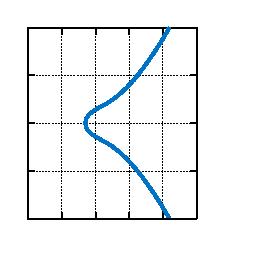
\includegraphics{implicit1}}%
    \gplfronttext
  \end{picture}%
\endgroup
}
\noindent Find $\dydx$ given the equation $x^3 + 3x + 2 = y^2$.\vspace{1mm}
\par\noindent\emph{Solution:} The above equation implicitly defines an
\emph{elliptic curve}\index{elliptic curve}, and its graph is shown on the
right. This curve is not a function $y=f(x)$, since it
violates the vertical line test, but $y$ still varies with $x$. To find
$\dydx$ take $\ddx$ of both sides of the equation then solve for $\dydx$:
\begin{align*}
\ddx\,(x^3 ~+~ 3x ~+~ 2) ~&=~ \ddx\,(y^2)\\[5pt]
3x^2 ~+~ 3 ~&=~ 2y \cdot \dydx \quad\text{by the Chain Rule, so}\\[5pt]
\dydx ~&=~ \frac{3x^2 ~+~ 3}{2y}
\end{align*}\vspace{-6mm}
\picskip{0}
At first this might seem unsatisfying---or confusing---since $\dydx$ is given
in terms of both $x$ and $y$. However, the derivative can still
be evaluated at specific points $(x,y)$ on the curve, i.e. any $(x,y)$
satisfying the original equation. For example, it is easy to check that
$(x,y) = (1,\sqrt{6})$ satisfies the equation $x^3 + 3x + 2 = y^2$, so
$\dydx(1,\sqrt{6}) = \frac{3(1)^2 + 3}{2\sqrt{6}} = \frac{\sqrt{6}}{2}$. Note
that $\dydx$ is not defined when $y=0$.

Notice that taking the square root of both sides of the original equation does
not result in an explicit formula for $y$, since $y = \pm \sqrt{x^3 + 3x + 2}$
defines \emph{two} functions, not just one. The beauty of implicit
differentiation is that the derivative $\dydx = \frac{3x^2 + 3}{2y}$ calculated
above gives you a single expression for the derivative of \emph{both} those
functions.
\end{exmp}
\divider
\newpage
An \emph{algebraic curve}\index{algebraic curve} is defined as the set of all
points $(x,y)$ satisfying a polynomial equation in the variables $x$ and $y$,
such as $x^2 - 3xy^4 + 1 = x^5 - y^2$. An \emph{elliptic curve} is a special
case of an algebraic curve, where the polynomial has the specific form
$x^3 + ax + b = y^2$, such as the equation $x^3 + 3x + 2 = y^2$ from Example
\ref{exmp:implicit1}. Elliptic curves have certain properties that have found
applications in cryptography.\footnote{For example, see Section 12.2 in
\textsc{Buchmann, J.A.}, \emph{Introduction to Cryptography}, New York:
Springer-Verlag, 2001.}

\begin{exmp}\label{exmp:implicit2}
\parpic[r]{% GNUPLOT: LaTeX picture with Postscript
\begingroup
\footnotesize
  \makeatletter
  \providecommand\color[2][]{%
    \GenericError{(gnuplot) \space\space\space\@spaces}{%
      Package color not loaded in conjunction with
      terminal option `colourtext'%
    }{See the gnuplot documentation for explanation.%
    }{Either use 'blacktext' in gnuplot or load the package
      color.sty in LaTeX.}%
    \renewcommand\color[2][]{}%
  }%
  \providecommand\includegraphics[2][]{%
    \GenericError{(gnuplot) \space\space\space\@spaces}{%
      Package graphicx or graphics not loaded%
    }{See the gnuplot documentation for explanation.%
    }{The gnuplot epslatex terminal needs graphicx.sty or graphics.sty.}%
    \renewcommand\includegraphics[2][]{}%
  }%
  \providecommand\rotatebox[2]{#2}%
  \@ifundefined{ifGPcolor}{%
    \newif\ifGPcolor
    \GPcolortrue
  }{}%
  \@ifundefined{ifGPblacktext}{%
    \newif\ifGPblacktext
    \GPblacktexttrue
  }{}%
  % define a \g@addto@macro without @ in the name:
  \let\gplgaddtomacro\g@addto@macro
  % define empty templates for all commands taking text:
  \gdef\gplbacktext{}%
  \gdef\gplfronttext{}%
  \makeatother
  \ifGPblacktext
    % no textcolor at all
    \def\colorrgb#1{}%
    \def\colorgray#1{}%
  \else
    % gray or color?
    \ifGPcolor
      \def\colorrgb#1{\color[rgb]{#1}}%
      \def\colorgray#1{\color[gray]{#1}}%
      \expandafter\def\csname LTw\endcsname{\color{white}}%
      \expandafter\def\csname LTb\endcsname{\color{black}}%
      \expandafter\def\csname LTa\endcsname{\color{black}}%
      \expandafter\def\csname LT0\endcsname{\color[rgb]{1,0,0}}%
      \expandafter\def\csname LT1\endcsname{\color[rgb]{0,1,0}}%
      \expandafter\def\csname LT2\endcsname{\color[rgb]{0,0,1}}%
      \expandafter\def\csname LT3\endcsname{\color[rgb]{1,0,1}}%
      \expandafter\def\csname LT4\endcsname{\color[rgb]{0,1,1}}%
      \expandafter\def\csname LT5\endcsname{\color[rgb]{1,1,0}}%
      \expandafter\def\csname LT6\endcsname{\color[rgb]{0,0,0}}%
      \expandafter\def\csname LT7\endcsname{\color[rgb]{1,0.3,0}}%
      \expandafter\def\csname LT8\endcsname{\color[rgb]{0.5,0.5,0.5}}%
    \else
      % gray
      \def\colorrgb#1{\color{black}}%
      \def\colorgray#1{\color[gray]{#1}}%
      \expandafter\def\csname LTw\endcsname{\color{white}}%
      \expandafter\def\csname LTb\endcsname{\color{black}}%
      \expandafter\def\csname LTa\endcsname{\color{black}}%
      \expandafter\def\csname LT0\endcsname{\color{black}}%
      \expandafter\def\csname LT1\endcsname{\color{black}}%
      \expandafter\def\csname LT2\endcsname{\color{black}}%
      \expandafter\def\csname LT3\endcsname{\color{black}}%
      \expandafter\def\csname LT4\endcsname{\color{black}}%
      \expandafter\def\csname LT5\endcsname{\color{black}}%
      \expandafter\def\csname LT6\endcsname{\color{black}}%
      \expandafter\def\csname LT7\endcsname{\color{black}}%
      \expandafter\def\csname LT8\endcsname{\color{black}}%
    \fi
  \fi
    \setlength{\unitlength}{0.0500bp}%
    \ifx\gptboxheight\undefined%
      \newlength{\gptboxheight}%
      \newlength{\gptboxwidth}%
      \newsavebox{\gptboxtext}%
    \fi%
    \setlength{\fboxrule}{0.5pt}%
    \setlength{\fboxsep}{1pt}%
\begin{picture}(2160.00,2160.00)%
    \gplgaddtomacro\gplbacktext{%
      \csname LTb\endcsname%
      \put(108,-4){\makebox(0,0){\strut{}$-3$}}%
      \csname LTb\endcsname%
      \put(378,-4){\makebox(0,0){\strut{}$-2$}}%
      \csname LTb\endcsname%
      \put(648,-4){\makebox(0,0){\strut{}$-1$}}%
      \csname LTb\endcsname%
      \put(918,-4){\makebox(0,0){\strut{}$0$}}%
      \csname LTb\endcsname%
      \put(1187,-4){\makebox(0,0){\strut{}$1$}}%
      \csname LTb\endcsname%
      \put(1457,-4){\makebox(0,0){\strut{}$2$}}%
      \csname LTb\endcsname%
      \put(1728,-4){\makebox(0,0){\strut{}$3$}}%
      \csname LTb\endcsname%
      \put(1860,216){\makebox(0,0)[l]{\strut{}$-3$}}%
      \csname LTb\endcsname%
      \put(1860,522){\makebox(0,0)[l]{\strut{}$-2$}}%
      \csname LTb\endcsname%
      \put(1860,828){\makebox(0,0)[l]{\strut{}$-1$}}%
      \csname LTb\endcsname%
      \put(1860,1134){\makebox(0,0)[l]{\strut{}$0$}}%
      \csname LTb\endcsname%
      \put(1860,1439){\makebox(0,0)[l]{\strut{}$1$}}%
      \csname LTb\endcsname%
      \put(1860,1745){\makebox(0,0)[l]{\strut{}$2$}}%
      \csname LTb\endcsname%
      \put(1860,2052){\makebox(0,0)[l]{\strut{}$3$}}%
    }%
    \gplgaddtomacro\gplfronttext{%
      \csname LTb\endcsname%
      \put(918,-243){\makebox(0,0){\strut{}$x$}}%
      \put(2133,1134){\makebox(0,0){\strut{}$y$}}%
    }%
    \gplbacktext
    \put(0,0){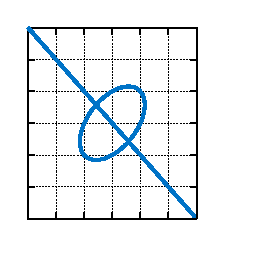
\includegraphics{implicit2}}%
    \gplfronttext
  \end{picture}%
\endgroup
}
\noindent Find $\dydx$ given the equation $x + y = x^3 + y^3$.\vspace{1mm}
\par\noindent\emph{Solution:} The above equation implicitly defines an
algebraic curve and its graph is shown on the right. To find
$\dydx$ take $\ddx$ of both sides of the equation then solve for $\dydx$:
\begin{align*}
\ddx\,(x ~+~ y) ~&=~ \ddx\,(x^3 ~+~ y^3)\\[6pt]
1 ~+~ \dydx ~&=~ 3x^2 ~+~ 3y^2 \cdot \dydx \quad\text{by the Chain Rule, so}\\[6pt]
\dydx ~&=~ \frac{3x^2 ~-~ 1}{1 ~-~ 3y^2}
\end{align*}\vspace{-9mm}
\picskip{0}
Notice that the curve consists of an oval shape (an ellipse, actually) with a
line through it. In fact,
that line is $y = -x$, as can be verified by replacing each instance of $y$ in
the equation $x + y = x^3 + y^3$ by $-x$ (resulting in the equation $0=0$). You
might be wondering how $\dydx$ is defined at the points where that line
intersects the ellipse: is it the slope of the line $y=-x$ (i.e. $-1$), or is it
the slope of the tangent line to the ellipse at those points (which would not
equal $-1$)? This is discussed in the exercises.

The graph was created with the free open-source graphing program
Gnuplot\footnote{See the documentation at
\url{http://www.gnuplot.info/documentation.html}} using the
following Gnuplot commands (which give an idea of how to plot implicit functions
in general):

\begin{Verbatim}[frame=single,framesep=3pt]
set size square
set view 0,0
set isosamples 500,500
set contour base
set cntrparam levels discrete 0
unset surface
set grid
unset key
unset ztics
set xlabel 'x'
set ylabel 'y'
f(x,y) = x + y - x**3 - y**3
splot [-3:3][-3:3] f(x,y) lw 3
\end{Verbatim}
\end{exmp}
\divider
\vspace{3mm}

\newpage
\begin{exmp}\label{exmp:implicitcir}
\parpic[r]{\begin{tikzpicture}[>=latex, every node/.style={font=\small}]
 \draw[->,black!60,line width=1pt] (-1.5,0) -- (1.8,0) node[right] {$x$};
 \draw[->,black!60,line width=1pt] (0,-1.2) -- (0,1.5) node[above] {$y$};
 \draw[linecolor,line width=1.5pt] (0,0) circle (1);
 \node[below left] at (0,0) {$0$}; 
 \node[below right] at (1,0) {$1$}; 
 \node[left] at (-0.4,1.2) {$x^2 + y^2 = 1$};
 \draw[red,line width=0.6pt] (0.8,0.6) -- +(-0.6,0.8) -- +(0.3,-0.4);
 \fill (0.8,0.6) circle (2.5pt);
 \node[right] at (0.8,0.6) {$(4/5,3/5)$};
\end{tikzpicture}}
\noindent Find the tangent line to the curve $x^2 + y^2 = 1$ at the point
$(4/5,3/5)$.\vspace{1mm}
\par\noindent\emph{Solution:} This curve is the unit circle, shown in the
picture on the right. First use implicit differentiation to find $\dydx$:
\begin{align*}
\ddx\,(x^2 ~+~ y^2) ~=~ \ddx\,(1) \quad&\Rightarrow\quad
2x ~+~ 2y \cdot \dydx ~=~ 0 \quad\text{by the Chain Rule}\\[4pt]
&\Rightarrow\quad \dydx ~=~ -\frac{x}{y}
\end{align*}\vspace{-7mm}
\picskip{0}
\noindent The slope $m$ of the tangent line to the curve at $(4/5,3/5)$ is then
$m = \dydx(4/5,3/5) = -\frac{4/5}{3/5} = -4/3$. Thus, the equation of the
tangent line is $y - \frac{3}{5} = -\frac{4}{3}\left(x - \frac{4}{5}\right)$.
\end{exmp}\vspace{-2mm}
\divider
\vspace{3mm}

\startexercises\label{sec3dot4}
{\small
\probs{A}

\par\noindent For Exercises 1-9, use implicit differentiation to find $\dydx$.

\begin{enumerate}[\bfseries 1.]
 \begin{multicols}{3}
  \item $x^3 y ~-~ 4xy^2 ~=~ y ~+~ x^2$
  \item $xy ~=~ (x+y)^3$
  \item $(x+y)^3 ~=~ (x - y + 1)^2$
 \end{multicols}
 \begin{multicols}{3}
  \item $x^{2/3} ~+~ y^{2/3} ~=~ a^{2/3}\vphantom{\dfrac{x}{x}}$
  \item $(x^2 - y^2 )^2 ~=~ 2x^2 + y^2\vphantom{\dfrac{x}{x}}$
  \item $\dfrac{x+y}{x-y} ~=~ x^2 + y^2$
 \end{multicols}
 \begin{multicols}{3}
  \item $\cos\,(xy) ~=~ \sin\,(x^2 y^2)$
  \item $x^3 ~-~ x ~=~ y^2$
  \item $x^3 y^2 e^{\sin\,(xy)} ~=~ x^2 ~+~ xy ~+~ y^3$
 \end{multicols}
  \item In Example \ref{exmp:implicitcir} is it possible to solve the equation
  $x^2 + y^2 = 1$ explicitly for $y$ in terms of $x$? Explain.
  \item In Example \ref{exmp:implicitcir} what happens to the tangent line
   at the point $(1,0)$? Why does this make sense geometrically?
  \item Find the equation of the tangent line to the curve
    $x^3 + 3x^2 y + y^3 ~=~ 8$ at the point $(2,0)$.
\suspend{enumerate}
\probs{B}
\resume{enumerate}[{[\bfseries 1.]}]
 \item Find $\frac{d^2y}{\dx^2}$ for the curve $x^2 + y^2 = 1$. You may use the
  results from Example \ref{exmp:implicitcir}.
 \item Show that at every point $(x_0,y_0)$ on the curve $y^2 = 4ax$, the
  equation of the tangent line to the curve is $y y_0 = 2a(x + x_0)$.
 \item\label{exer:elliptan} Show that at every point $(x_0,y_0)$ on the ellipse
  $\dfrac{x^2}{a^2} + \dfrac{y^2}{b^2} = 1$,
  the equation of the  tangent line to the ellipse is
  $\dfrac{x x_0}{a^2} + \dfrac{y y_0}{b^2} = 1$.
 \item\label{exer:hyptan} Show that at every point $(x_0,y_0)$ on the hyperbola
  $\dfrac{x^2}{a^2} - \dfrac{y^2}{b^2} = 1$,
  the equation of the  tangent line to the hyperbola is
  $\dfrac{x x_0}{a^2} - \dfrac{y y_0}{b^2} = 1$.
 \item Show that $\dydx$ is not defined at the points of intersection of the
  line and ellipse described by the curve $x+y=x^3+y^3$ from Example
  \ref{exmp:implicit2}. \emph{(Hint: Factor the equation $x+y=x^3+y^3$.)}
 \item Show that the points $P=(2,4)$ and $Q=(-31/64,-337/512)$ are on the
  elliptic curve $x^3+3x+2=y^2$ from Example \ref{exmp:implicit1}, and that the
  tangent line to the curve at $P$ also goes through $Q$.
\end{enumerate}
}
\newpage
%Begin Section 3.5
\section{Related Rates}
If several quantities are related by an equation, then differentiating both
sides of that equation with respect to a variable (usually $t$, representing
time) produces a relation between the rates of change of those quantities.
The known rates of change are then used in that relation to determine an
unknown related rate.\index{related rates}

\begin{exmp}\label{exmp:relrate1}
\parpic[r]{\begin{tikzpicture}[>=latex, every node/.style={font=\small}]
 \fill[fillcolor] (0,0) -- (2,0) -- (4,1.5) -- (4,2.5) -- (2,2.5)
  -- (0,1) -- cycle;
 \draw[line width=1.5pt] (0,0) -- (2,0) node[midway,below] {$100$} -- (4,1.5)
  node[midway,below right] {$300$} -- (4,3) -- (2,3) -- (0,1.5) -- cycle;
 \draw[line width=1.5pt] (0,1.5) -- (2,1.5) -- (4,3);
 \draw[line width=1.5pt] (2,1.5) -- (2,0);
 \draw[dashed] (0,1) -- (2,1) -- (4,2.5) -- (2,2.5) -- cycle;
 \draw[dashed] (0,0) -- (2,1.5) -- (4,1.5);
 \draw[dashed] (2,1.5) -- (2,2.5);
 \draw[line width=1.5pt] (2,2.5) -- (2,3);
 \draw[|<->|] (4.4,1.5) -- (4.4,3) node[midway,fill=white] {$10$};
 \draw[|<->|] (-0.4,0) -- (-0.4,1) node[midway,fill=white] {$h$};
\end{tikzpicture}}
\noindent Suppose that water is being pumped into a rectangular pool at a rate
of 60,000 cubic feet per minute. If the pool is 300 ft long, 100 ft wide, and
10 ft deep, how fast is the height of the water inside the pool changing?\vspace{1mm}
\par\noindent\emph{Solution:} Let $V$ be the volume of the water in the pool.
Since the volume of a rectangular solid is the product of the length, width, and
height of the solid, then
\[
V ~=~ (300)(100)h ~=~ 30000h ~~\text{ft}^3
\]
where $h$ is the height of the water, as in the picture on the right.
Both $V$ and $h$ are functions of time $t$ (measured in minutes), and
$\dVdt = 60000~\text{ft}^3$/min was given. The goal is to find
$\frac{d\!h}{\dt}$. Since
\[
\dVdt ~=~ \ddt\,(30000h) ~=~ 30000\,\frac{d\!h}{\dt}
\]
then
\[
\frac{d\!h}{\dt} ~=~ \frac{1}{30000} \dVdt ~=~ \frac{1}{30000}\cdot 60000
~=~ 2~\text{ft/min} .
\]
\end{exmp}
\begin{exmp}\label{exmp:relrate2}
\parpic[r]{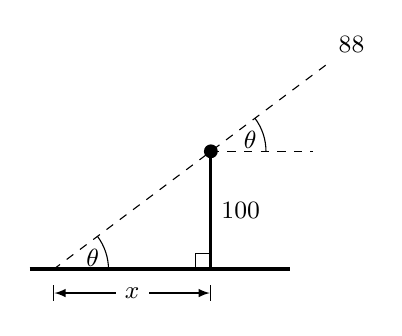
\begin{tikzpicture}[>=latex, every node/.style={font=\small}]
 \draw[line width=1.5pt] (-0.3,0) -- (3,0);
 \draw[line width=1pt] (2,0) -- (2,1.5) node[midway,right] {$100$};
 \fill (2,1.5) circle (2.5pt);
 \draw[dashed] (0,0) -- (3.5,2.625) node[above right] {\ding{88}};
 \draw[|<->|] (0,-0.3) -- (2,-0.3) node[midway,fill=white] {$x$};
 \draw[dashed] (2,1.5) -- (3.3,1.5);
 \draw (1.8,0) -- (1.8,0.2) -- (2,0.2);
 \node at (0.5,0.15) {$\theta$};
 \draw (0.7,0) arc (0:36.86:0.7);
 \node[shift={(2,1.5)}] at (0.5,0.15) {$\theta$};
 \draw[shift={(2,1.5)}] (0.7,0) arc (0:36.86:0.7);
\end{tikzpicture}}
\noindent Suppose that the angle of inclination from the top of a 100 ft pole
to the sun is decreasing at a rate of $0.05$ radians per minute. How fast is the
length of the pole's shadow on the ground increasing when the angle of
inclination is $\pi/6$ radians? You may assume that the pole is perpendicular to
the ground.\vspace{1mm}
\par\noindent\emph{Solution:} Let $\theta$ be the angle of inclination and let
$x$ be the length of the shadow, as in the picture on the right. Both $\theta$
and $x$ are functions of time $t$ (measured in minutes), and
$\frac{d\negmedspace\theta}{\dt} = -0.05$ rad/min was given (the derivative is
negative since $\theta$ is decreasing). The goal is to find $\dxdt$ when
$\theta = \pi/6$, denoted by $\dxdt\Biggr|_{\theta=\pi/6}$ (the vertical bar
means ``evaluated at'' the value of the subscript to the right of the bar).
Since
\[
x ~=~ 100\;\cot\,\theta \quad\Rightarrow\quad
\dxdt ~=~ -100\;\csc^2\theta \cdot \frac{d\negmedspace\theta}{\dt}
~=~ -100\;\csc^2\theta \cdot (-0.05) ~=~ 5\;\csc^2\theta
\]
then
\[
\dxdt\Biggr|_{\theta=\pi/6} ~=~ 5\;\csc^2(\pi/6) ~=~ 5\;(2)^2 ~=~ 20~\text{ft/min} .
\]
\end{exmp}
\divider
\newpage
\begin{exmp}\label{exmp:relrate3}
\noindent The radius of a right circular cylinder is decreasing at the rate of
$3$ cm/min, while the height is increasing at the rate of $2$ cm/min. Find the
rate of change of the volume of the cylinder when the radius is $8$ cm and the
height is $6$ cm.\vspace{1mm}
\par\noindent\emph{Solution:} Let $r$, $h$, and $V$ be the radius, height, and
volume, respectively, of the cylinder. Then $V = \pi\,r^2 \,h$. Since
$\frac{\dr}{\dt} = -3$ cm/min and $\frac{d\negmedspace h}{\dt} = 2$ cm/min, then
by the Product Rule:
\[
  \dVdt ~=~ \ddt (\pi\,r^2 \,h) ~=~ \left( 2\pi \,r\;\cdot\;\drdt\right)\,h ~+~
  \pi\,r^2 \;\cdot\;\frac{d\negmedspace h}{\dt} \quad\Rightarrow\quad
  \dVdt\Biggr|_{\text{\scriptsize{$\begin{matrix}r=8\\h=6\end{matrix}$}}} ~=~
  2\pi\,(8)\,(-3)\,(6) ~+~ \pi\,(8^2)\,(2) ~=~
 -160\pi~\frac{\text{\scriptsize cm}^3}{\text{\scriptsize min}}
\]
\end{exmp}
\divider
\vspace{2mm}
 
\startexercises\label{sec3dot5}
{\small
\probs{A}
\begin{enumerate}[\bfseries 1.]
 \item A stone is dropped into still water. If the radius of the circular outer
  ripple increases at the rate of $4$ ft/s, how fast is the area of the circle
  of disturbed water increasing when the radius is $10$ ft?
 \item The radius of a sphere decreases at a rate of 3 mm/hr. Determine how fast
  the volume and surface area of the sphere are changing when the radius is 5 mm.
 \item A kite $80$ ft above level ground moves horizontally at a rate of
  $4$ ft/s away from the person flying it. How fast is the string being
  released at the instant when $100$ ft of string have been released?
 \item A $10$-ft ladder is leaning against a wall on level ground. If the
  bottom of the ladder is dragged away from the wall at the rate of $5$ ft/s,
  how fast will the top of the ladder descend at the instant when it is $8$ ft
  from the ground?
 \item A person $6$ ft tall is walking at a rate of $6$ ft/s away from a light
  which is $15$ ft above the ground. At what rate is the end of the person's
  shadow moving along the ground away from the light?
 \item An object moves along the curve $y = x^3$ in the $xy$-plane. At what
  points on the curve are the $x$ and $y$ coordinates of the object changing at
  the same rate?
 \item The radius of a right circular cone is decreasing at the rate of $4$
  cm/min, while the height is increasing at the rate of $3$ cm/min. Find the
  rate of change of the volume of the cone when the radius is $6$ cm and
  the height is $7$ cm.
 \item Two boats leave the same dock at the same time, one goes north at
  25 mph and the other goes east at 30 mph. How fast is the distance between
  the boats changing when they are 100 miles apart?
 \item Repeat Exercise 8 with the angle between the boats being $110\Degrees$.
\suspend{enumerate}
\probs{B}
\resume{enumerate}[{[\bfseries 1.]}]
 \item An angle $\theta$ changes with time. For what values of $\theta$
  do $\sin\,\theta$ and $\tan\,\theta$ change at the same rate?
 \item Repeat Example \ref{exmp:relrate2} but with the ground making a
  $100\Degrees$ angle with the pole to the left of the pole.
\suspend{enumerate}
\probs{C}
\resume{enumerate}[{[\bfseries 1.]}]
 \item An upright cylindrical tank full of water is tipped over at a
 constant angular speed. Assume that the height of the tank
 is at least twice its radius. Show that at the instant the tank has
 been tipped $45\Degrees$, water is leaving the tank twice as fast as it did
 at the instant the tank was first tipped.
 \emph{(Hint: Think of how the water looks inside the tank as it is being tipped.)}
\end{enumerate}
}
\newpage
%Begin Section 3.6
\section{Differentials}
An \emph{ideal gas}\index{ideal gas} satisfies the equation $PV \;=\; RT$,
where $R$ is a constant and $P$, $V$, and $T$ are the pressure, volume per
mole, and temperature, respectively, of the gas. It will be proved that
\begin{equation}\label{eqn:gaslaw}
 \dfrac{\dP}{P} ~+~ \dfrac{\dV}{V} ~=~ \dfrac{\dT}{T} ~.
\end{equation}
Recall that $\dP$, $\dV$, and $\dT$ represent infinitesimal changes in the
quantities $P$, $V$, and $T$, respectively. Notice that none of the quotients in
Equation (\ref{eqn:gaslaw}) have an infinitesimal in the denominator. For example,
$\dP$ is divided not by $\dx$ or $\dt$, as it would be in a derivative such as
$\frac{\dP}{\dx}$ or $\frac{\dP}{\dt}$. Instead it is divided by $P$, which is not
an infinitesimal. So Equation (\ref{eqn:gaslaw}) is an equation that relates
infinitesimals themselves, i.e. infinitesimal changes, not infinitesimal
\emph{rates} of change. This is, in fact, how many physical laws are stated, for
reasons that will be discussed shortly.

Though infinitesimals have been used
throughout this text, many calculus textbooks\footnote{More accurately, many
\emph{current} calculus textbooks never mention them. Calculus texts up through
the 1930s or so not only mentioned infinitesimals but used them extensively,
even to the point of the texts themselves having titles such as \emph{Introduction
to Infinitesimal Calculus}.} do not even mention them, instead preferring to call
them \emph{differentials}.\footnote{Though often in an unclear and sometimes
confusing and misleading manner, as will be seen later in this section.} For
compatibility, the definition is given here:

\statedefn{defn:differential}{For a differentiable function $f(x)$, the
\textbf{differential} of $f(x)$ is\index{differential}
\begin{equation}\label{eqn:differential}
\df ~=~ f'(x)\;\dx
\end{equation}
where $\dx$ is an infinitesimal change in $x$.}
Note that this is identical to Equation (\ref{eqn:dffprimedx}) in Section 1.3.

\begin{exmp}\label{exmp:diff1}
\noindent Find the differential $\df$ of $f(x) = x^3$.\vspace{1mm}
\par\noindent\emph{Solution:} By definition,
\[
\df ~=~ f'(x)\;\dx ~=~ 3x^2\;\dx
\]
Equivalently, this can be written as
\[
d(x^3) ~=~ 3x^2\;\dx ~,
\]
which is often the way it would appear in textbooks in the sciences.
\end{exmp}
\divider
\vspace{3mm}

All the rules for derivatives (e.g. sum rule, product rule) apply to
differentials, and can be proved simply by multiplying the corresponding
derivative rule by $\dx$ on both sides of the equation:
\newpage
\statethm{thm:differentials}{Let $f$ and $g$ be differentiable functions, and
let $c$ be a constant. Then:
\begin{enumerate}[\bfseries (a)]
 \item $d(c) ~= 0$
 \item $d(cf) ~=~ c\,\df$ \quad(Constant Multiple Rule)
 \item $d(f + g) ~=~ \df ~+~ \dg$ \quad(Sum Rule)
 \item $d(f - g) ~=~ \df ~-~ \dg$ \quad(Difference Rule)
 \item $d(fg) ~=~ f\,\dg ~+~ g\,\df$ \quad(Product Rule)
 \item $d\left(\dfrac{f}{g}\right) ~=~ \dfrac{g\,\df ~-~ f\,\dg}{g^2}$ \quad(Quotient Rule)
 \item $d(f^n) ~=~ nf^{n-1}\,\df$ \quad(Power Rule)
 \item $d(f(g)) ~=~ \dfrac{\df}{\dg}\;\dg$  \quad(Chain Rule)
\end{enumerate}
}
For example, to prove (e), multiply both sides of the usual Product Rule by
$\dx$ so that
\begin{align*}
\frac{d(fg)}{\dx} ~=~ f\,\frac{\dg}{\dx} ~+~ g\,\frac{\df}{\dx} \quad&\Rightarrow\quad
 d(fg) ~=~ \cancel{\dx}\,\left(f\,\frac{\dg}{\cancel{\dx}} ~+~
 g\,\frac{\df}{\cancel{\dx}}\right)\\
&\Rightarrow\quad d(fg) ~=~ f\,\dg ~+~ g\,\df \quad\checkmark
\end{align*}
since the $\dx$ terms all cancel. The proofs of the other rules are similar.

The differential version of the ideal gas law in Equation (\ref{eqn:gaslaw})
\[
 \dfrac{\dP}{P} ~+~ \dfrac{\dV}{V} ~=~ \dfrac{\dT}{T}
\]
can now be proved by taking the differential of both sides of the equation $PV = RT$:
\begin{align*}
 d(PV) ~&=~ d(RT) ~=~ R \cdot \dT \quad\text{by the Constant Multiple Rule}\\
 V \; \dP ~+~ P \; \dV ~&=~ \frac{PV}{T} \; \dT \quad\text{by the Product Rule and since
 $R = \frac{PV}{T}$}\\[6pt]
 \frac{V\;\dP}{PV} ~+~ \frac{P\;\dV}{PV} ~&=~ \frac{\dT}{T} \quad\text{after dividing both
 sides by $PV$}\\[6pt]
 \frac{\dP}{P} ~+~ \frac{\dV}{V} ~&=~ \frac{\dT}{T} \quad\checkmark
\end{align*}
Notice that $\frac{\dP}{P}$, $\frac{\dV}{V}$ and $\frac{\dT}{T}$ represent
the \emph{relative} infinitesimal changes in $P$, $V$, and $T$, respectively.
The differential formulation is useful for finding one relative infinitesimal
change when the other two are known.

\begin{exmp}\label{exmp:diff2}
\noindent Suppose that $M$ is the total mass of a rocket and its unburnt fuel
at any time $t$ (so $M$ is a function of $t$). Over an infinitesimal time $\dt$
a mass $\dm$ of fuel is burnt and the gas byproducts are expelled out the rear
of the rocket at a velocity $v_E$ relative to the rocket. Using the law of
conservation of momentum over the interval $\dt$, show that
\[
 v_E\,\dm ~=~ M\,\dv
\]
where $m$ and $v$ are the mass of burnt fuel and the velocity of the rocket,
respectively, at the beginning of the time $\dt$.\vspace{1mm}
\par\noindent\emph{Solution:} Momentum is defined as mass times velocity.
The momentum of the rocket at the beginning of the time $\dt$ is thus $Mv$.
At the end of the time $\dt$, the momentum of the rocket consists of two parts,
namely the momentum of the rocket and its remaining unburnt fuel, which is
\begin{gather}
\text{((mass before $\dt$) $-$ (increase in burnt fuel)) $\times$
((velocity before $\dt$) $+$ (increase in velocity))}\\
(M - \dm)(v + \dv)
\end{gather}
and the momentum of the fuel that was burnt and expelled out the rear, which is
\[
(v - v_E)\,\dm ~.
\]
So by conservation of momentum,
\begin{align*}
Mv ~&=~ (M - \dm)(v + \dv) ~+~ (v - v_E)\,\dm\\
Mv ~&=~ Mv ~-~ v\,\dm ~+~ M\,\dv ~-~ (\dm)(\dv) ~+~ v\,\dm ~-~ v_E\,\dm, \quad\text{so}\\
 v_E\,\dm ~&=~ M\,\dv ~-~ (\dm)(\dv) ~=~ M\,\dv
\end{align*}
since $(\dm)(\dv) = (m'(t)\,\dt)(v'(t)\,\dt) ~=~ m'(t)v'(t)(\dt)^2 
~=~ m'(t)v'(t) \cdot 0 = 0$.\vspace{2mm}

\noindent Dividing both sides of $v_E\,\dm = M\,\dv$ by $\dt$ yields the equation
\[
M\,\dot{v} ~=~ \dot{m}\,v_E
\]
using the dot notation---mentioned in Section 1.3---for the derivative with
respect to the time variable $t$, which is still popular with physicists. Since
$\dot{v}$ is just acceleration $a$, this formulation is the classic equation for
the acceleration of a rocket.\footnote{For other formulations see Chapter 1 in
\textsc{Rosser, J.B., R.R. Newton and G.L. Gross}, \emph{Mathematical Theory of
Rocket Flight}, New York: McGraw-Hill Book Company, Inc., 1947.}
\end{exmp}
\divider
\vspace{3mm}

Letting $f$ be the natural logarithm function and letting $g = u$ in the
differential version of the Chain Rule yields the following useful result:

\statethm{thm:dlnu}{\begin{center}
$d(\ln\,u) ~=~ \dfrac{\du}{u}$
\end{center}}
This is often used in a differential version of the technique of logarithmic
differentiation\index{logarithmic differentiation} discussed in Section 2.3.

\begin{exmp}\label{exmp:diff3}
\noindent Prove the relation $\frac{\dP}{P} + \frac{\dV}{V} = \frac{\dT}{T}$
using logarithmic differentiation.\vspace{1mm}
\par\noindent\emph{Solution:} Take the natural logarithm and then the differential
of both sides of the equation $PV = RT$:
\begin{align*}
\ln\,(PV) ~=~ \ln\,(RT) \quad&\Rightarrow\quad
\ln\,P ~+~ \ln\,V ~=~ \ln\,R ~+~ \ln\,T\\
&\Rightarrow\quad d(\ln\,P ~+~ \ln\,V) ~=~ d(\ln\,R ~+~ \ln\,T)\\
&\Rightarrow\quad \frac{\dP}{P} ~+~ \frac{\dV}{V} ~=~ 0 ~+~ \frac{\dT}{T} ~=~ \frac{\dT}{T}
\quad\text{(since $\ln\,R$ is a constant)}
\end{align*}
\end{exmp}
\begin{exmp}\label{exmp:diff4}
\noindent The derivative of the area $\pi r^2$ of a circle of radius
  $r$, as a function of $r$, equals its circumference $2\pi r$. Use the notion
  of a differential as an infinitesimal change to explain why this makes sense
  geometrically.\vspace{1mm}
\par\noindent\emph{Solution:} Let $A = \pi r^2$ be the area of a circle of
varying radius $r$. Then $A'(r) = 2\pi r$, which is equivalent to saying
$d\negmedspace A = 2\pi r\,\dr$. To see why this makes sense geometrically,
imagine increasing the radius by $\dr$, as in the picture below on the left.
This increases the area $A$ of the circle to $A + d\negmedspace A$, with
$d\negmedspace A$ the infinitesimal area of the shaded ring in the picture.

\begin{center}
\begin{tikzpicture}[every node/.style={font=\small}]
 \filldraw[fill=fillcolor,line width=1pt] (0,0) circle (2);
 \filldraw[fill=white,line width=1pt] (0,0) circle (1.5);
 \draw[-latex] (0,0) -- (0,1.5) node[midway,right] {$r$};
 \draw[dashed] (0,1.5) -- (0,2) node[midway,right] {$\dr$};
 \draw[line width=2.5pt,-latex] (3,1) -- (4.8,1)
  node[midway,above,align=left] {slice and\\roll flat};
 \node at (1.75,0) {$d\negmedspace A$};
 \fill (0,0) circle (2.5pt);
 \begin{scope}[>=latex,shift={(7,1)}]
  \filldraw[fill=fillcolor,line width=1pt] (0,0) -- (6,0) -- (5.5,0.5) -- (0.5,0.5) --cycle;
  \draw[|<->|] (0.5,0.8) -- (5.5,0.8) node[fill=white,midway] {$2\pi r$};
  \draw[|<->|] (0,-0.3) -- (6,-0.3) node[fill=white,midway] {$2\pi(r+\dr)$};
  \draw[dashed] (0.5,0) -- (0.5,0.5) node[midway,right] {$\dr$};
  \draw[dashed] (5.5,0) -- (5.5,0.5);
  \node at (3,0.25) {area $= d\negmedspace A$};
 \end{scope}
 \begin{scope}[shift={(5.5,-1.5)}]
  \filldraw[fill=fillcolor,line width=1pt] (0,0) -- (1.5,0) node[midway,below] {$\pi\;\dr$}
   -- (1.5,1.5) node[midway,right] {$\dr$} -- cycle;
  \draw (1.3,0) -- (1.3,0.2) -- (1.5,0.2);
  \draw[line width=1.5, latex-] (2.3,0.75) -- (3,0.75) node[right] {area $= 0$};
 \end{scope}
\end{tikzpicture}
\end{center}

Slice that ring along the dashed line then roll it flat, yielding a trapezoid
with height $\dr$, top length $2\pi r$ (from the circumference of the inner
circle of the ring), and bottom length $2\pi(r+\dr)$ (from the circumference of
the outer circle of the ring), as shown in the picture above on the right. The
triangular edges of the trapezoid contribute nothing to the area of the
trapezoid, since (by the Microstraightness Property) the hypotenuse of each is
indeed a straight line, so each is a right triangle with height $\dr$ and (by
symmetry) base $\pi\dr$, thus having area $\frac{1}{2}\pi(\dr)^2 = 0$. Hence the
entire area $d\negmedspace A$ of the trapezoid comes from the rectangular
portion of height $\dr$ and base $2\pi r$, which means
$d\negmedspace A = 2\pi r\,\dr$, as expected.
\end{exmp}
\divider
\vspace{3mm}

The above example answers the question of whether it is a happy coincidence that
the derivative of a circle's area turns out to be the circle's
circumference---no, it is not! Some other such cases (e.g. the derivative of a
sphere's volume is its surface area) are left to the exercises. Note that a
similar ``coincidence'' does \emph{not} occur for a square: if $x$ is the length
of each side then the area is $x^2$, but the derivative of $x^2 $ is $2x$, which
is \emph{not} the perimeter of the square (i.e. $4x$). Why does this not follow
the same pattern as the circle? Think about a key difference in the shape of a
square in comparison to a circle, keeping differentiability in mind.

There are many benefits to using differentials---i.e. infinitesimals---in
calculus.\footnote{For an excellent overview on this subject, see \textsc{Dray,
T. and C.A. Manogue}, Putting Differentials Back into Calculus,
\emph{College Math. J.} \textbf{41} (2010), 90\symbol{45}100. Some of the
material in this section is indebted to that paper, which is available at
\url{http://www.math.oregonstate.edu/bridge/papers/differentials.pdf}} For
example, recall Example \ref{exmp:relrate3} in Section 3.5 on related rates,
where the volume $V$ of a right circular cylinder with radius $r$ and height
$h$ changes with time $t$ as
\[
\dVdt ~=~ \left( 2\pi \,r\;\cdot\;\drdt\right)\,h ~+~
 \pi\,r^2 \;\cdot\;\frac{d\negmedspace h}{\dt} ~.
\]
The above equation forces you to consider only the derivative with respect
to the time variable $t$. What if you wanted to see the rates of change with
respect to another variable, such as $r$, $h$, or some other quantity?
In that case using the differential version of the above equation, namely
\[
\dV ~=~ 2\pi \,rh\;\dr ~+~ \pi\,r^2 \;d\negmedspace h
\]
provides more flexibility---you are free to divide both sides by any
differential, not just by $\dt$. Many related rates problems would likely
benefit from this approach.

Present-day calculus textbooks confuse the notion of a differential
(infinitesimal) $\dx$ with the idea of a small but real value $\Delta x$. The
two are \emph{not} the same. An infinitesimal is \emph{not} a real number and
\emph{cannot} be assigned a real value, no matter how small; $\Delta x$
\emph{can} be assigned real values. Using $\dx$ and $\Delta x$
interchangeably is a source of much confusion for students (likewise for $\dy$
and $\Delta y$). This confusion rears its head in exercises involving the
linear approximation of a curve by its tangent line near a point $x_0$, namely
$f(x) \approx f(x_0) + f'(x_0)(x - x_0)$ when $x-x_0$ is ``small'' (e.g.
$\sqrt{63} \approx 7.9375$, by using $f(x)=\sqrt{x}$, $x=63$, $x_0=64$, and
$x-x_o = \Delta x = -1$).
Such exercises have nothing to do with differentials, not to mention having
dubious value nowadays. They are remnants of a bygone era, before the advent of
modern computing obviated the need for such (generally) poor
approximations.\\\vspace{2mm}
\divider
\vspace{3mm}

\startexercises\label{sec3dot6}
{\small
\probs{A}
\begin{enumerate}[\bfseries 1.]
 \begin{multicols}{2}
 \item Find the differential $\df$ of $f(x) = x^2 - 2x + 5$.
 \item Find the differential $\df$ of $f(x) = \sin^2 (x^2)$.
 \end{multicols}
 \begin{multicols}{2}
 \item Show that $d\left(\tan^{-1}(y/x)\right) = \dfrac{x\,\dy ~-~ y\,\dx}{x^2 ~+~ y^2}$
 \item Given $y^2 - xy + 2x^2 = 3$, find $\dy\vphantom{\dfrac{x\,\dy ~-~ y\,\dx}{x^2 ~+~ y^2}}$.
 \end{multicols}
 \item The \emph{elasticity}\index{elasticity} of a function $y = f(x)$ is
 $E(y) = \dfrac{x}{y} \cdot \dfrac{\dy}{\dx}~$. Show that $E(y) = \dfrac{d(\ln\,y)}{d(\ln\,x)}~$.
 \item Prove the differential version of the Quotient Rule:
 \[
  d\left(\dfrac{f}{g}\right) ~=~ \dfrac{g\,\df ~-~ f\,\dg}{g^2}
 \]
\newpage
 \item Let $y = c\,u^n$, where $c$ and $n$ are constants. Show that
 \[
  \frac{\dy}{y} ~=~ n\,\frac{\du}{u} ~.
 \]
 \item Obviously the derivative of the constant $\pi^2$ is not $2\pi$. But is
  $d(\pi^2) = 2\pi\,d(\pi)$ true? Explain.
\suspend{enumerate}
\probs{B}
\resume{enumerate}[{[\bfseries 1.]}]
 \item The \emph{continuity relation} for an ideal gas is
 \[
 \frac{PM}{\sqrt{T}} ~=~ \text{constant}
 \]
 where $P$ and $T$ are the pressure and temperature, respectively, of the gas,
 and $M$ is the \emph{Mach number}\index{Mach number}. Show that
 \[
 \frac{\dP}{P} ~+~ \frac{d\!M}{M} ~=~ \frac{\dT}{2T} ~.
 \]
 \item For an ideal gas, satisfying the equation $PV = RT$ as before, the \emph{Gibbs
  energy} $G$ is defined as $G = H - TS$, where $H$ and $S$ are
  the \emph{enthalpy} and \emph{entropy}, respectively, of the gas.\index{Gibbs energy}
  \begin{enumerate}[\bfseries (a)]
   \item Show that
   \begin{displaymath}
    d\left(\dfrac{G}{RT}\right) ~=~ \dfrac{1}{RT}\,dG ~-~ \dfrac{G}{RT^2}\,\dT ~.
   \end{displaymath}
   \item One of the \emph{fundamental property relations} for an ideal gas
    (which you do not need to prove) is\index{enthalpy}\index{entropy}
    \begin{displaymath}
     dG ~=~ V\,\dP ~-~ S\,\dT ~.
    \end{displaymath}
    Use this and part (a) to show that
   \begin{displaymath}
    d\left(\dfrac{G}{RT}\right) ~=~ \dfrac{V}{RT}\,\dP ~-~ \dfrac{H}{RT^2}\,\dT ~.
   \end{displaymath}
  \end{enumerate}
 \item The derivative of the volume $\pi r^2 h$ of a right circular cylinder of
  radius $r$ and height $h$, as a function of $r$, equals its lateral surface
  area $2\pi r h$. Use the notion of a differential as an infinitesimal change
  to explain why this makes sense geometrically.
 \item The derivative of the volume $\frac{4\pi}{3}r^3$ of a sphere of radius
  $r$, as a function of $r$, equals its surface area $4\pi r^2$. Use the notion
  of a differential as an infinitesimal change to explain why this makes sense
  geometrically.
 \item In \emph{quantum calculus}\index{quantum calculus} the
  \emph{$q$-differential}\index{q-differential@$q$-differential} of a function
   $f(x)$ is
\[
d_qf(x) ~=~ f(qx) ~-~ f(x) ~,
\]
and the \emph{$q$-derivative}\index{q-derivative@$q$-derivative} of $f(x)$ is
\[
D_qf(x) ~=~ \frac{d_qf(x)}{d_qx} ~=~ \frac{f(qx) ~-~ f(x)}{qx ~-~ x} ~=~
\frac{f(qx) ~-~ f(x)}{(q - 1)x} ~.
\]
\begin{enumerate}[\bfseries (a)]
 \item Show that for all positive integers $n$,
\[
D_q\left(x^n\right) ~=~ \lbrack n \rbrack\, x^{n-1} ~,
\]
where $\lbrack n \rbrack = 1 + q + q^2 + \cdots + q^{n-1}$.
 \item Use part (a) to show that for all positive integers $n$,
\[
\lim_{q \to 1}~D_q\left(x^n\right) ~=~ \ddx\left(x^n\right) ~.
\]
\end{enumerate}
\end{enumerate}
}
